%(Aquí lo dejaría con la estructura que teníamos para Caise, presentamos el framework y posteriormente comentamos modelos y transformaciones)

This section presents \pisodm, an MDD-based methodology for building service compositions with non-functional requirements. 
\pisodm provides meta-models for modelling functional and non-functional requirements organized in three levels (Figure~\ref{fig:piSOD-M}): CIM (\textit{Computational Independent Models}), PIM (\textit{Platform Independent Models}) and PSM (\textit{Platform Specific Models}). 
Given  high-level models specified at the CIM level, \pisodm proposes the semi-automatic refinement of these models, for the generation  of a set of models at the other levels of abstraction.
The refinement process is driven by transformation rules specified between the meta-models.
\begin{figure}[h]
\centering
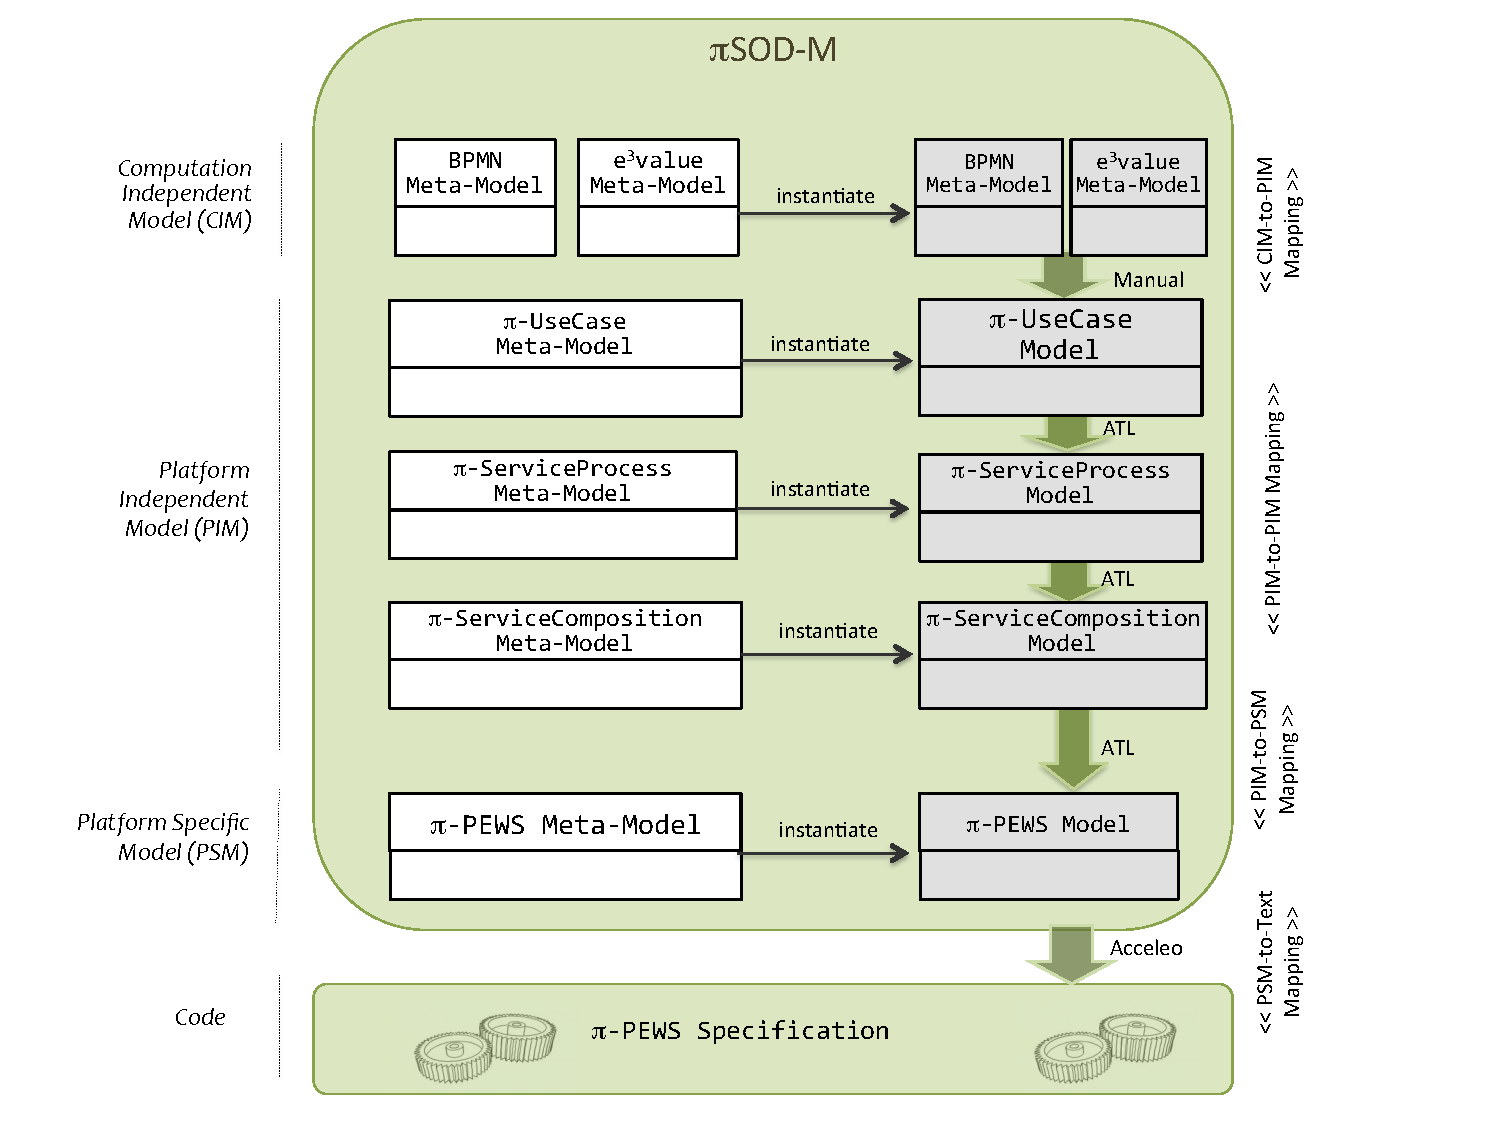
\includegraphics[width=1.0\textwidth]{figs/piSOD-M_process.pdf}
\caption{$\pi$SOD-M Overview.}
\label{fig:piSOD-M}
\end{figure}



%. . - -. . - -. . - -. . - -. . - -. . - -. . - -. . - -. . - -. . - -. . - -. . - -. . - -. . - -. . - -. . - -. . - -. . - -. . - -. . - -. . - -. . - -. . - -. . - -. . - -. . - -
\subsection{Computation Independent Models}
%. . - -. . - -. . - -. . - -. . - -. . - -. . - -. . - -. . - -. . - -. . - -. . - -. . - -. . - -. . - -. . - -. . - -. . - -. . - -. . - -. . - -. . - -. . - -. . - -. . - -. . - -

This level focusses on the highest-level view of the system, including its business and requirement specifications.
At this stage of the development, the structure and system processing details are still unknown or undetermined.  
\pisodm uses the \textit{e$^3$value}~\cite{Gordijn02valuebased} and \textit{BPMN}~\cite{BPMN} meta-models for this purpose. 

% .   .  .   .  .   .  .   .  .   .  .   .  .   .  .   .  .   .  .   .  .   .  .   .  .   .  .   .  .   .  .   .  .   .  .   .  .   .  .   .  .   .  .   .  .   .  .   .  .   .  .   .  .   .  .   .  .   .   
\subsubsection{E$^3$value meta-model}
% .   .  .   .  .   .  .   .  .   .  .   .  .   .  .   .  .   .  .   .  .   .  .   .  .   .  .   .  .   .  .   .  .   .  .   .  .   .  .   .  .   .  .   .  .   .  .   .  .   .  .   .  .   .  .   .  .   . 

The e$^3$value model of an application identifies the value/information exchange between components of the system. 
It is a business model that represents a business case graphically as a set of value exchanges\footnote{See Figure~\ref{fig:CIM:tpme3v}.} ($\nabla$ $\triangle$) and value activities (rounded boxes) performed by business actors (squared boxes).
The model is well suited to enhance the understanding of the environment in which an application is being developed. 
It defines \textit{dependency paths}, showing the value exchange between providers and end users when they ask for a service.
A dependency path has a direction and consists of a sequence of linked dependency nodes.
It starts with a \textit{start stimulus} node and ends with an \textit{end stimulus} node (see Figure~\ref{fig:CIM:tpme3v}). 
Dependency paths may also contain \textsl{OR} and \textsl{AND} elements (both for initiate and join alternative and parallel paths).

\begin{figure}[htpb]
\center
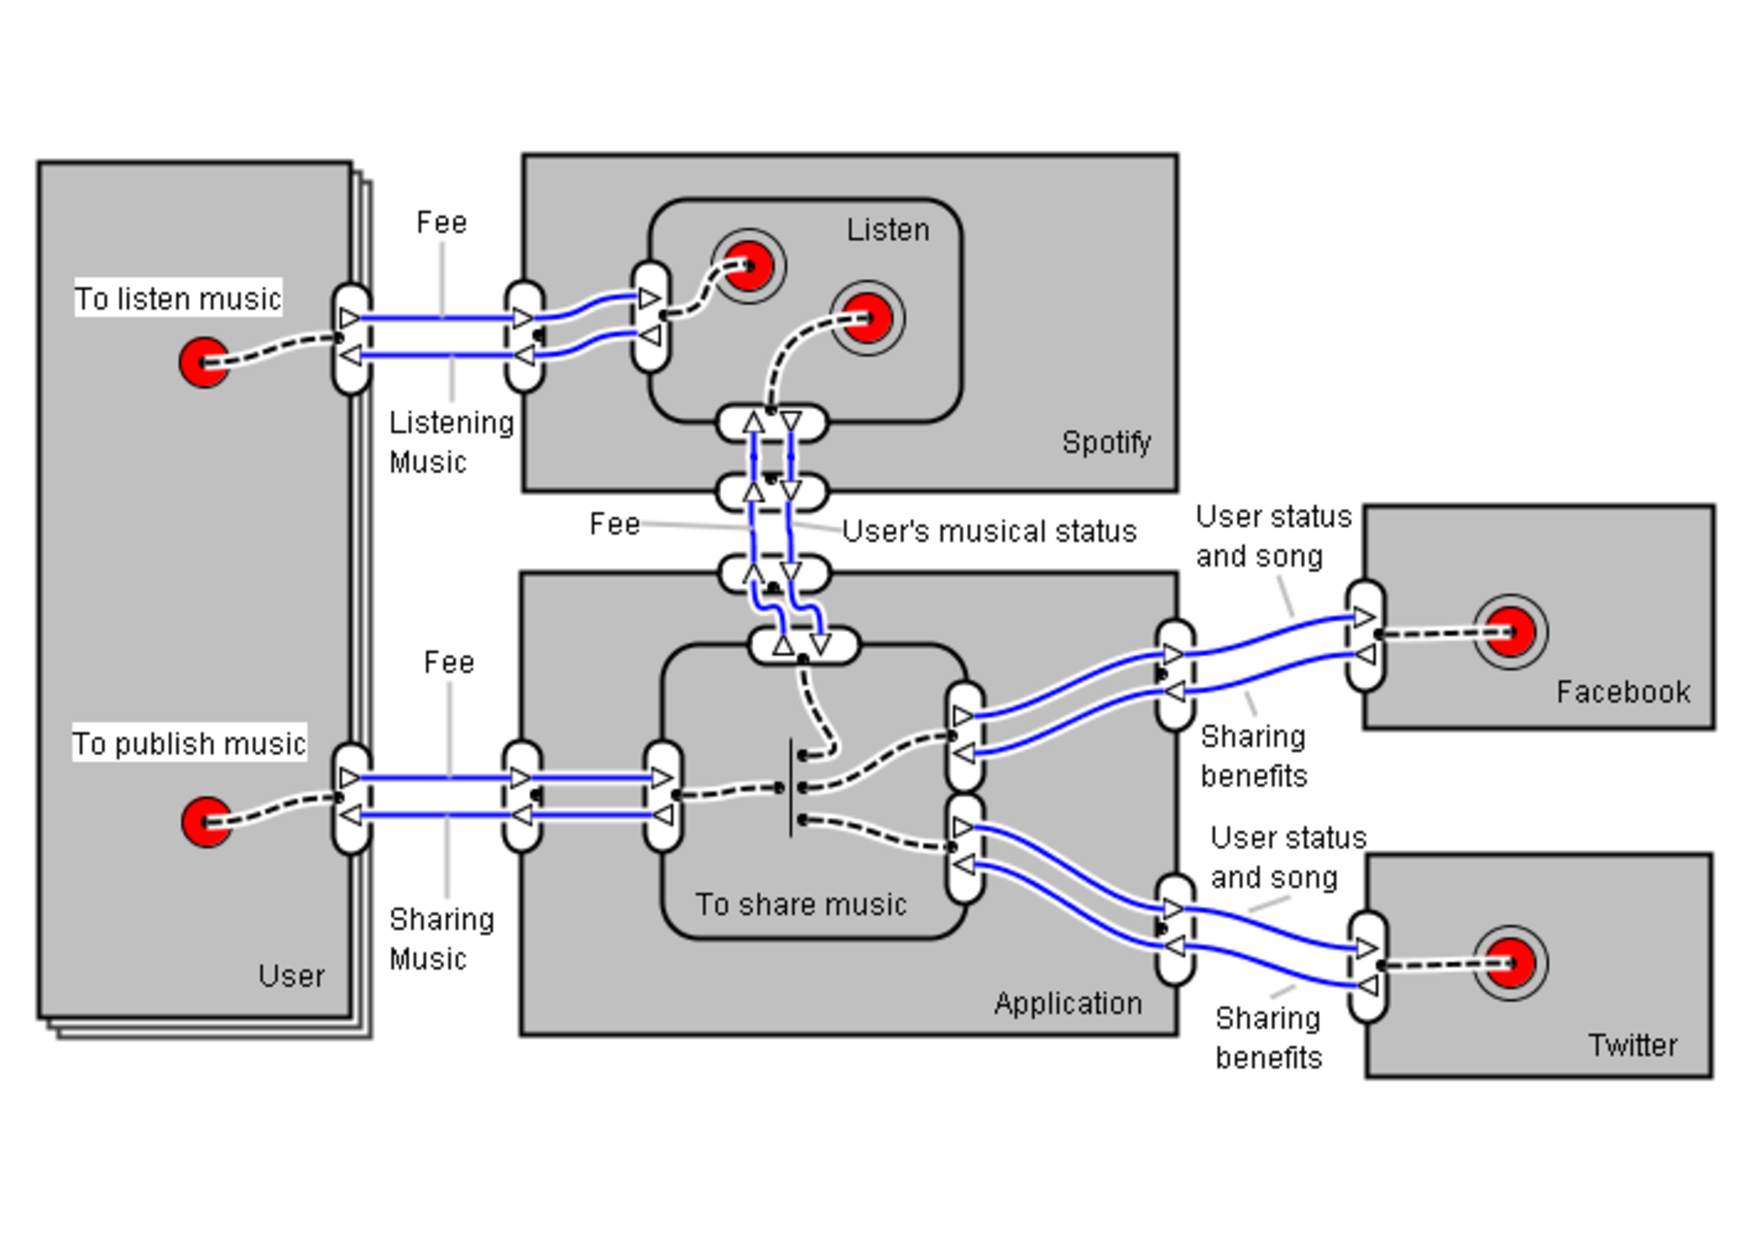
\includegraphics[width=0.75\textwidth]{figs/e3value.pdf}
\hspace*{5cm}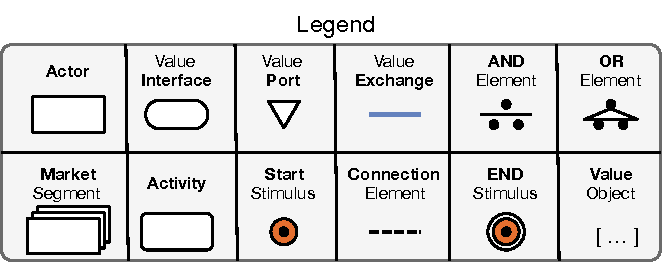
\includegraphics[width=0.4\textwidth]{figs/3ValueKey.pdf}
\caption{\label{fig:CIM:tpme3v} e3value model for ``To Publish Music''.}
\end{figure}

\begin{example}[To Publish Music]\label{ex:toPublicMusic}
Let us consider the scenario ``To Publish Music'', which will be used as a running example in this section:
An organization wants to provide the service based application ``To Publish Music'' that monitors the music listened by a user during some periods of time and sends the song title  to this person's Twitter and Facebook accounts. 
In this way, this social network user will have her status synchronized in  Twitter and Facebook (i.e., either the same title is published in both accounts or it is not updated) with the title of the music she is listening in Spotify.
The application is based on three external actors ({\em Spotify, Twitter} and {\em Facebook}).
The following (external) services will be used by the application:
\begin{itemize}
\item The music service   Spotify exports a method for obtaining information  about the music a given user is listening:
\begin{itemize} \item {\sf\small get-Last-Song ( userid ): String} ; \end{itemize}
\item Facebook and Twitter services export methods for  updating the status of a given user:
\begin{itemize} 
%\item{\sf\small get-Status ( usedid ): String ; 
\item {\sf\small update-Status ( userid, new-status ): String}; 
\end{itemize}
\end{itemize}




The e$^3$value model for ``To Publish Music'' is shown in Figure~\ref{fig:CIM:tpme3v}. 
The e$^3$value value model shows Spotify and a private application (which is also a service) that directly interact with users for providing free services for listening and publishing information about music being listened by users. The private application interacts with Spotify for obtaining free information about the flow of music being listened by a user in return of a fee (i.e., premium subscription). Finally, the private application interacts with Facebook and Twitter for updating the user's status.
We can see this interaction as non material benefit sharing (as users subscribe to their networks and are active on them thanks to the private application).
\end{example}

The e$^3$value  model is used to model the (economic) value exchange among the actors involved in an application. It is also necessary to understand the business process of the application and the conditions in which the different steps of this process are executed input/out data and the dependencies among these steps. Therefore, our methodology proposes the BPMN meta-model as a tool for modeling this aspect of the application.


%Note that the models at this level show\dots 
%{\color{red} Valeria and Placido: Please explain the CIM models for this example.}
%\hfill\openbox
% .   .  .   .  .   .  .   .  .   .  .   .  .   .  .   .  .   .  .   .  .   .  .   .  .   .  .   .  .   .  .   .  .   .  .   .  .   .  .   .  .   .  .   .  .   .  .   .  .   .  .   .  .   .  .   .  .   . 
\subsubsection{BPMN meta-model}% .   .  .   .  .   .  .   .  .   .  .   .  .   .  .   .  .   .  .   .  .   .  .   .  .   .  .   .  .   .  .   .  .   .  .   .  .   .  .   .  .   .  .   .  .   .  .   .  .   .  .   .  .   .  .   .  .   . 
BPMN~\cite{BPMN}  is a graphical representation that establishes the business process of the application through a high-level workflow. 
The next example illustrates the use of this meta-model.

\begin{example}[To Publish Music \textit{(cont)}]\label{ex:toPublicMusicBPMN}
Figure \ref{fig:CIM:tpmbpmn} shows the BPMN model\footnote{Details on BPMN (Business Process Management Notation) can be found in http://www.bpmn.org/} of the scenario. 
It starts by contacting the music service Spotify for retrieving the user's  musical status (activity {\sf Get Song}). 
Twitter and Facebook services are then contacted in parallel for updating the user's status with the corresponding song title (activities {\sf Update Twitter} and {\sf Update Facebook}).
\end{example}
%
\begin{figure}[htpb]
\center
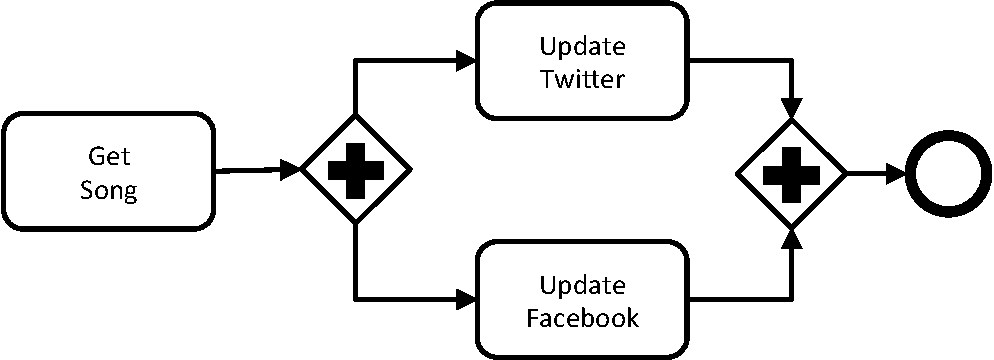
\includegraphics[width=0.49\textwidth]{figs/SC.pdf}
\caption{\label{fig:CIM:tpmbpmn} BPMN model for ``To Publish Music''.}
\end{figure}

The CIM level models are the basis for the development of the application. 
The information presented at this level is (manually) refined into PIM-level models of the methodology \pisodm described next.
Notice tat, at this level, the models are (very informally) used to describe both functional and non-functional requirements.

%. . - -. . - -. . - -. . - -. . - -. . - -. . - -. . - -. . - -. . - -. . - -. . - -. . - -. . - -. . - -. . - -. . - -. . - -. . - -. . - -. . - -. . - -. . - -. . - -. . - -. . - -
\subsection{Platform Independent Models}
%. . - -. . - -. . - -. . - -. . - -. . - -. . - -. . - -. . - -. . - -. . - -. . - -. . - -. . - -. . - -. . - -. . - -. . - -. . - -. . - -. . - -. . - -. . - -. . - -. . - -. . - -

This level focusses on the system functionality, hiding the details of any particular platform.
The specification defines those parts of the system that do not change from one platform to another. 
Our methodology defines three PIM-level meta-models: \textit{$\pi$-UseCase}, \textit{$\pi$-ServiceProcess} and \textit{$\pi$-ServiceComposition}.
 
 % .   .  .   .  .   .  .   .  .   .  .   .  .   .  .   .  .   .  .   .  .   .  .   .  .   .  .   .  .   .  .   .  .   .  .   .  .   .  .   .  .   .  .   .  .   .  .   .  .   .  .   .  .   .  .   .  .   . 
\subsubsection{\textit{$\pi$-UseCase} meta-model}% .   .  .   .  .   .  .   .  .   .  .   .  .   .  .   .  .   .  .   .  .   .  .   .  .   .  .   .  .   .  .   .  .   .  .   .  .   .  .   .  .   .  .   .  .   .  .   .  .   .  .   .  .   .  .   .  .   . 

Figure~\ref{fig:CIM:usecasemetamodel} presents the \textit{$\pi$-UseCase} meta-model.
The goal of \textit{$\pi$-UseCase}  is to be the first representation of the application in terms of functionality, as well as to represent its non-functional requirements.
The notion of \textit{policy} is used to describe NFRs. 
(In Figure~\ref{fig:CIM:usecasemetamodel}, we have highlighted the concepts related to NFRs).
The \textit{$\pi$-UseCase} meta-model extends the UML Use Case meta-model for describing non-functional requirements with  the concepts:  {\sc Business service}, {\sc End consumer}, {\sc Requirement}, {\sc Use Case}, {\sc Composite Use Case}, {\sc non-functional requirement}, {\sc non-functional attribute} and {\sc Constraint}. An {\sc End Consumer} is represented by an {\sc Actor}. An  {\sc Actor} is related to {\sc Use Cases} (from the original UML definition), while a {\sc  Composite Use Case} is a set of actions performed by the system which can be broken into different {\sc Use Cases}.
{\sc  Business Service} aggregates several {\sc Use Cases},  a service can be expressed by one or more use cases.
 The {\sc Business Collaborators} concept are represented  through {\sc Packages}. A {\sc Business Collaborator} represents an external service or a system that interact with the application that are being modelled. Each {\sc Business Collaborators} combines the features described in each  {\sc Package}. Thus, the services functions can be
specified being grouped into packages.
 
 \begin{figure}[htpb]
\center
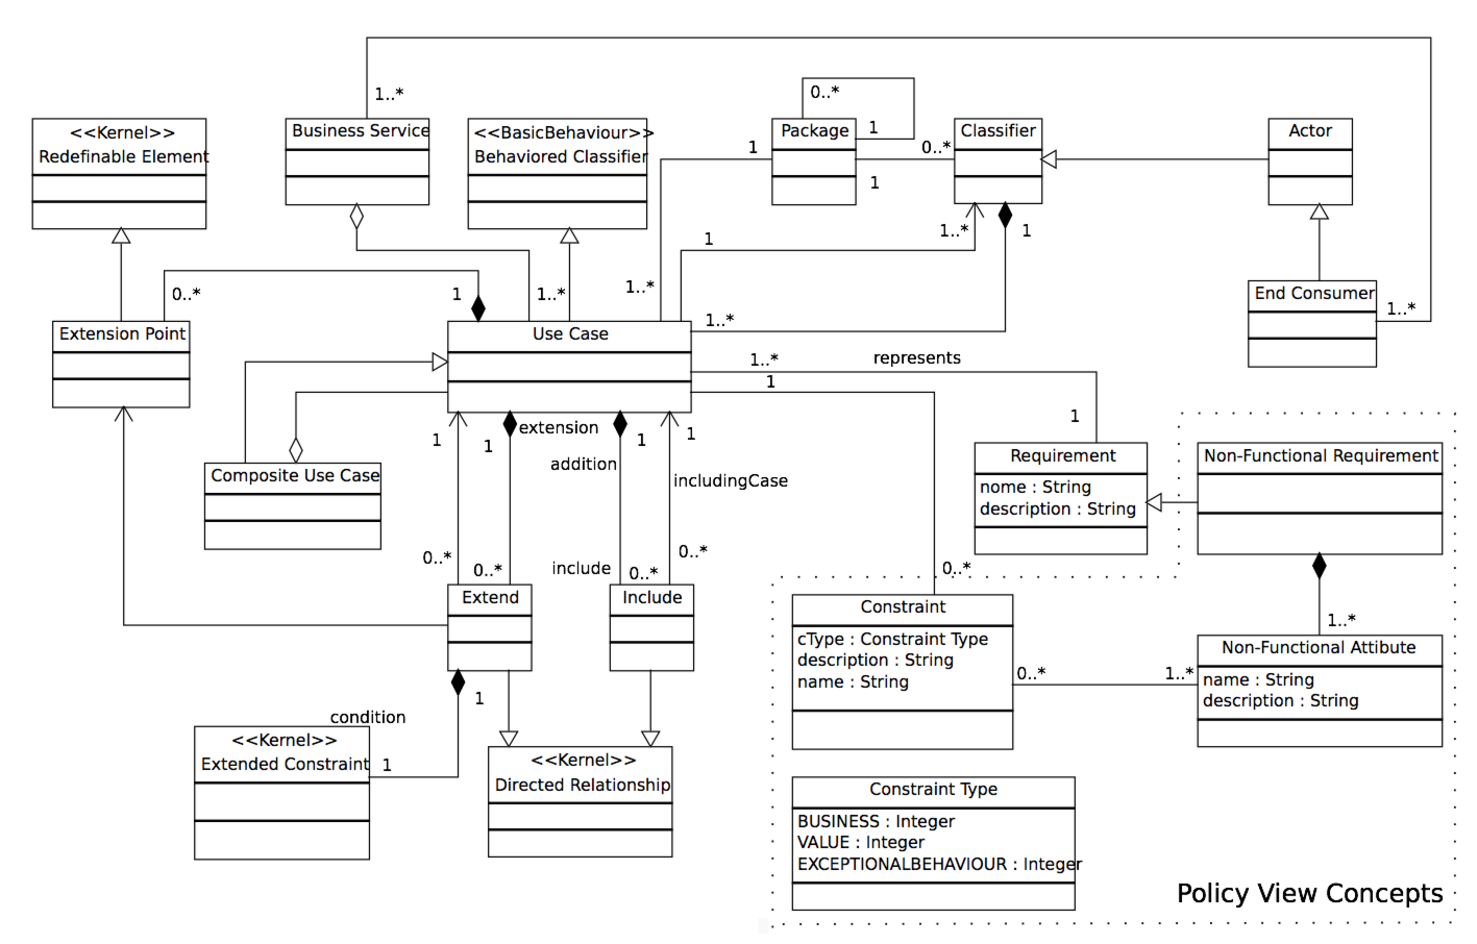
\includegraphics[width=0.9\textwidth]{figs/UseCaseMetaModel.pdf}
\caption{\label{fig:CIM:usecasemetamodel} $\pi$-UseCase Meta-Model.}
\end{figure}


 The {\sc Non-functional requirement} and {\sc Non-functional Attribute} concepts are represented as part of description of {\sc Use Cases} and {\sc Constraints}. 
A {\sc Use Case} may have several {\sc Constraints}. Each {\sc Constraint} has its name, description, and which ones should be checked during the execution of the application. Each {\sc Constraint} is represented as a stereotyped ({\sf �constraint�}) use case. A restriction may be associated to data ({\sc Value Constraint}), represented as the stereotype �value�; it can represent business rules (Business Constraint), represented as the stereotype {\sf �business�}; and it can represent {\sc Exceptional Behaviour} constraints, represented as the stereotype {\sf �exceptional\_behaviour�}.
 We use part of our case study to illustrate this meta-model. 
 \begin{example}[To Publish Music \textit{(cont)}]\label{ex:toPublicMusic2}
Figure~\ref{fig:CIM:piusecasetpm} shows a $\pi$-UseCase model for our example application.
We consider that, besides the service composition for implementing the application, it is necessary to model  other requirements that represent the (i) conditions imposed by services usage --for example, the fact that both Facebook and Twitter require authentication protocol in order to call their methods for updating the wall; (ii) the conditions stemming from the business rules of the application logic, (e.g., the fact that the walls in Facebook and Twitter must show the same song title and if this is not possible then none of them is updated). 
 
The ``To Publish Music'' use case expects  the Facebook or Twitter user status to be changed every time a user starts listening a new song.
  Therefore, it is necessary to perform a social network authentication with the users data. Each social network uses different services and different forms of authentication. The authentication constraint is required to update a music status. The restriction is stereotyped as a �value� constraint, because the users id and password are verified.  Figure \ref{fig:CIM:piusecasetpm} shows the buy music, download music, listen music and pay use cases. The process of buying a song requires the user private data for a Spotify account, and also a secure connection, represented as �value� and �business� constraint, respectively. For payment, the user must provide the data of payment card or PayPal account login and password, represented as �value� stereotype. Other restriction is that the minimum payment value is 2 euros.
%{\color{red} Talk about this model for the example.}
\end{example}

\begin{figure}[htpb]
\center
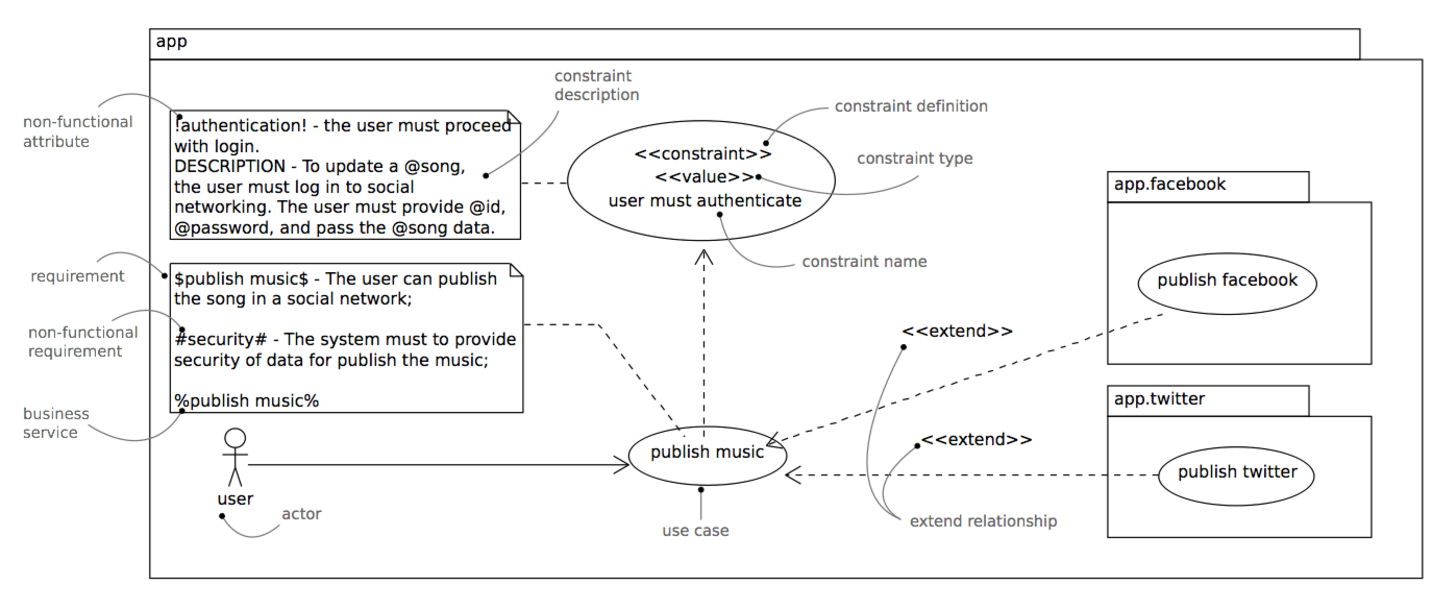
\includegraphics[width=0.9\textwidth]{figs/UseCase.pdf}
\caption{\label{fig:CIM:piusecasetpm} $\pi$-UseCase model for ``To Publish Music''.}
\end{figure}
 

 % .   .  .   .  .   .  .   .  .   .  .   .  .   .  .   .  .   .  .   .  .   .  .   .  .   .  .   .  .   .  .   .  .   .  .   .  .   .  .   .  .   .  .   .  .   .  .   .  .   .  .   .  .   .  .   .  .   . 
\subsubsection{\textit{$\pi$-ServiceProcess} meta-model}% .   .  .   .  .   .  .   .  .   .  .   .  .   .  .   .  .   .  .   .  .   .  .   .  .   .  .   .  .   .  .   .  .   .  .   .  .   .  .   .  .   .  .   .  .   .  .   .  .   .  .   .  .   .  .   .  .   . 

The \textit{$\pi$-ServiceProcess} meta-model extends the UML activity diagram with the concept of \textit{contract} to represent constraints over data and actions. This concept is used to model 
groups  of  constraints described in the \textit{$\pi$-UseCase}. 
As shown in Figure~\ref{fig:CIM:serviceprocessmetamodel}, the concepts of the \textit{$\pi$-ServiceProcess} meta-model are: {\sc Contract}, {\sc Assertion}, {\sc Exceptional behaviour}, {\sc Activity}, {\sc Service Activity}, {\sc Action} and {\sc Constraint}.
The highlighted portion of the figure corresponds to the concepts related to the representation of NFRs.

A specific \textit{$\pi$-ServiceProcess} model shows the set of logically related activities to be performed in a service-based application. 
So, the activities of this model represent a behaviour that is part of the business logic of the application. 
A \textit{$\pi$-ServiceProcess}  model contains three main elements: (i) service process, (ii) service activity and (iii) activity contract. A service activity represents an operation that is part of the execution flow, and it is modelled as an {\sc Action}. 
An activity contract represents the {\sc Non-functional Requirement}  that is also part of the execution flow of a service, identified  as a stereotyped activity ({\sf �assertion�}). 
The {\sc Assertion}s associated to an {\sc Action} compose a {\sc Contract}. Using the concepts {\sc Contract} and {\sc Assertion} it is possible to specify each activity service, by defining its pre-conditions and post-conditions.

\begin{figure}[htpb]
\center
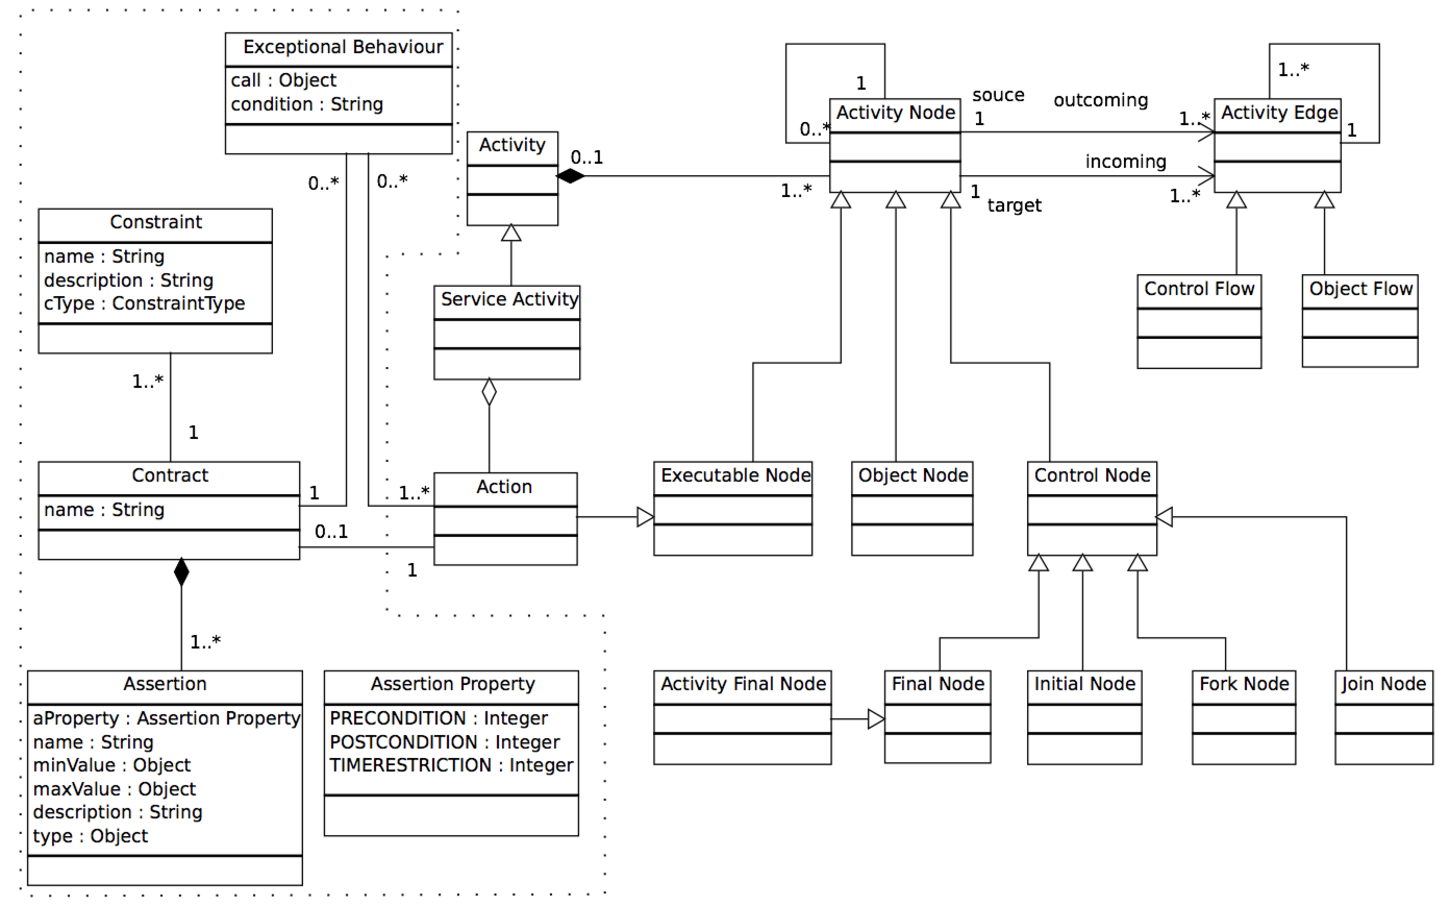
\includegraphics[width=0.9\textwidth]{figs/ServiceProcessMetaModel.pdf}
\caption{\label{fig:CIM:serviceprocessmetamodel} $\pi$-Service Process Meta-Model.}
\end{figure}

%According to the meta-model, a \textit{$\pi$-ServiceProcess} model represents the service processes and its contracts. It models the set of system activities and describe contracts for each activity or the process as a whole. Each service identified in the previous model (\textit{$\pi$-UseCase}) is mapped to an action. This model defines a workflow for  modeling business logic and the behaviour of the application being developed. The behaviour is represented by each action and the restrictions by the assertion description. All assertions are described by stereotyped actions.

\begin{example}[To Publish Music \textit{(cont)}]\label{ex:toPublicMusic3}
Considering the example scenario, the contract based process of activities  is shown in figure \ref{fig:CIM:serviceprocess}. The buy music and publish music services (update Twitter and Facebook) have pre- and post-conditions assertions that are composed into a contract for each service. The buy music pre-conditions consist in verifying: 
(i) if the User data are correct; 
(ii) if the User is already logged in Spotify; 
(iii) if bank account information are correct and; 
(iv) if there are enough funds in the bank account to cover the payment. 
A post-condition ensures the complete transaction and verifies if a notification was sent to the user and Spotify, about the payment authorization. There are four assertions for the buy music action, and each assertion has been detailed with the assertion property and predicate that must be verified. To update services, depending of each service, there may be different restrictions. As an example, a new verification of user data and message format is appropriate (maximum 140 characters), in case of Twitter. In the case of Facebook, it is required that the user is already logged on Spotify and these data are the same as Facebook. 
As post-condition, the application ensures that the Facebook service sends a notification of success. 
To update Twitter a pre-condition is required, while to update Facebook it is necessary to check a pre-condition and a confirmation notice (modelled as post-condition). 
As a pre-condition for ``twitter update'' it is necessary that (i) the music format be correct and (ii) the twitter login and password be correct for the update.
\end{example}

\begin{figure}[htpb]
\center
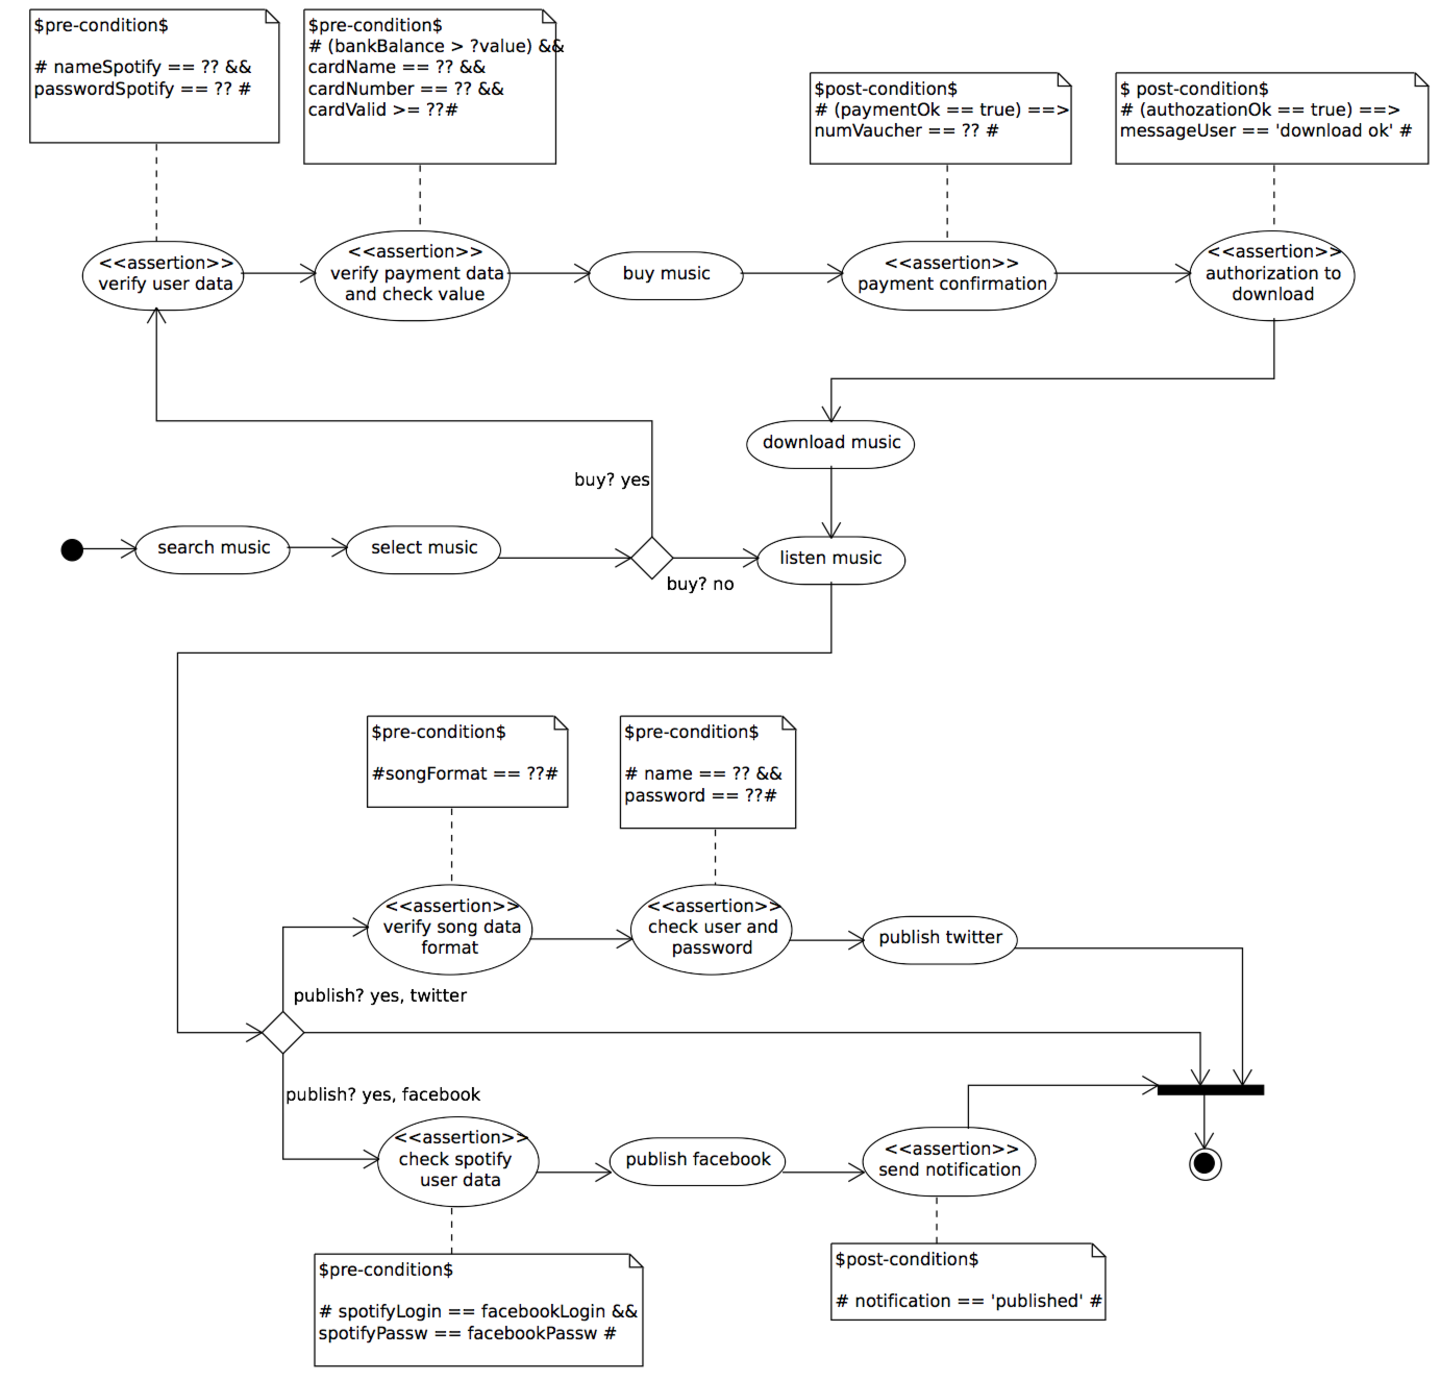
\includegraphics[width=0.9\textwidth]{figs/ServiceProcess.pdf}
\caption{\label{fig:CIM:serviceprocess} $\pi$-ServiceProcess model for ``To Publish Music''.}
\end{figure}

% .   .  .   .  .   .  .   .  .   .  .   .  .   .  .   .  .   .  .   .  .   .  .   .  .   .  .   .  .   .  .   .  .   .  .   .  .   .  .   .  .   .  .   .  .   .  .   .  .   .  .   .  .   .  .   .  .   . 
\subsubsection{\textit{$\pi$-ServiceComposition} meta-model}% .   .  .   .  .   .  .   .  .   .  .   .  .   .  .   .  .   .  .   .  .   .  .   .  .   .  .   .  .   .  .   .  .   .  .   .  .   .  .   .  .   .  .   .  .   .  .   .  .   .  .   .  .   .  .   .  .   . 

As shown in Figure \ref{fig:e-scomposition-metamodel}, the $\pi$-Serv\-ice\-Com\-po\-si\-tion meta-model 
provides meta-classes to represent workflows\footnote{Workflows will be transformed into implemented service compositions.} that model  business processes.
The \textit{$\pi$-Serv\-ice\-Com\-po\-si\-tion} meta-model extends the UML activity  meta-model with the concept of  \textit{A-Policy}
to group contracts with similar non-functional requirements.
For instance, security and privacy restrictions may be grouped into a security policy.
 The  ($\pi$-Serv\-ice\-Com\-po\-si\-tion) meta-model defines:
%In the meta-model of Figure~\ref{fig:e-scomposition-metamodel}:
\begin{itemizedTrivlist}
\item A {\sc Business Collaborator} meta-class, to represent the classes of entities that collaborate in  business processes by performing some  required action. 
An instance of this meta-class is graphically represented as a partition in the activity diagram. 
A collaborator can be either internal or external to the system. 
When the collaborator of the business is external to the system, the attribute {\sf IsExternal}\footnote{We use the {\sf sans serif} font for referring to classes defined using a meta-model.} of the collaborator is set to \textbf{true}.

\item {\sc Action}s, a kind of {\sc ExecutableNode}, are represented in the model as a class activity instance of the meta-class \textsc{Action}. 
A class action represents some type of transformation or processing. 
There are two types of actions: i) a WebService (attribute Type is {\sf WS}); and ii) a simple operation called an {\sc ActivityOperation} (attribute Type is {\sc AOP}).
\begin{figure}[t]
\centering
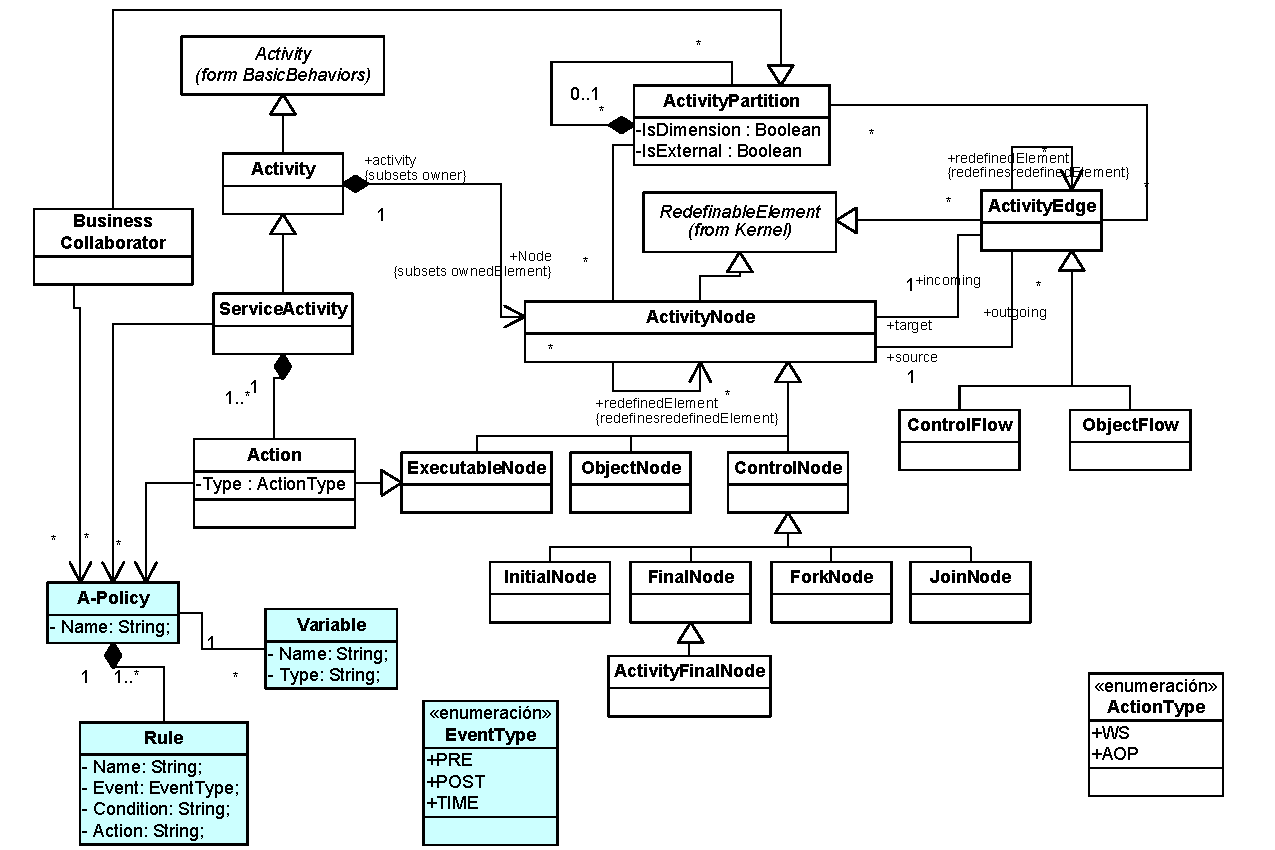
\includegraphics[width=1.0\textwidth]{figs/E-service-composition-metamodel}
\caption{$\pi$-Service Composition Metamodel.}
\label{fig:e-scomposition-metamodel}
\end{figure}

\item The {\sc ServiceActivity} meta-class represents classes of composite activity types that must be carried out as part of a business service and is composed by one or more executable nodes.

\item In order to represent constraint types associated to services compositions, we introduced the meta-classes {\sc Rule} and {\sc A-policy} (see blue meta-classes in the $\pi$-Serv\-ice\-Com\-po\-si\-tion meta-model in Figure \ref{fig:e-scomposition-metamodel}).
We model non-functional constraints by using the notion of {\em A-policy}~\cite{Espinosa-Oviedo2011a,CIC:eovszmc09c}.
An {\em A-policy} is defined by attributes and rules. 
Intuitively, the conditions of each rule will be evaluated.
In case of no compliance, the actions defined by the rule will be performed.
The {\sc Rule} meta-class represents the types of event-condition-action rules where the {\sc Event} part represents the moment in which a constraint  will be evaluated.
An {\em A-policy} defines variables and operations that can be shared by the rules and that can be used for expressing their Event and Condition parts. 
\end{itemizedTrivlist}
Instances of this meta-model are represented as UML activity diagrams. 
\begin{figure}[t]%[htpb]
\centering
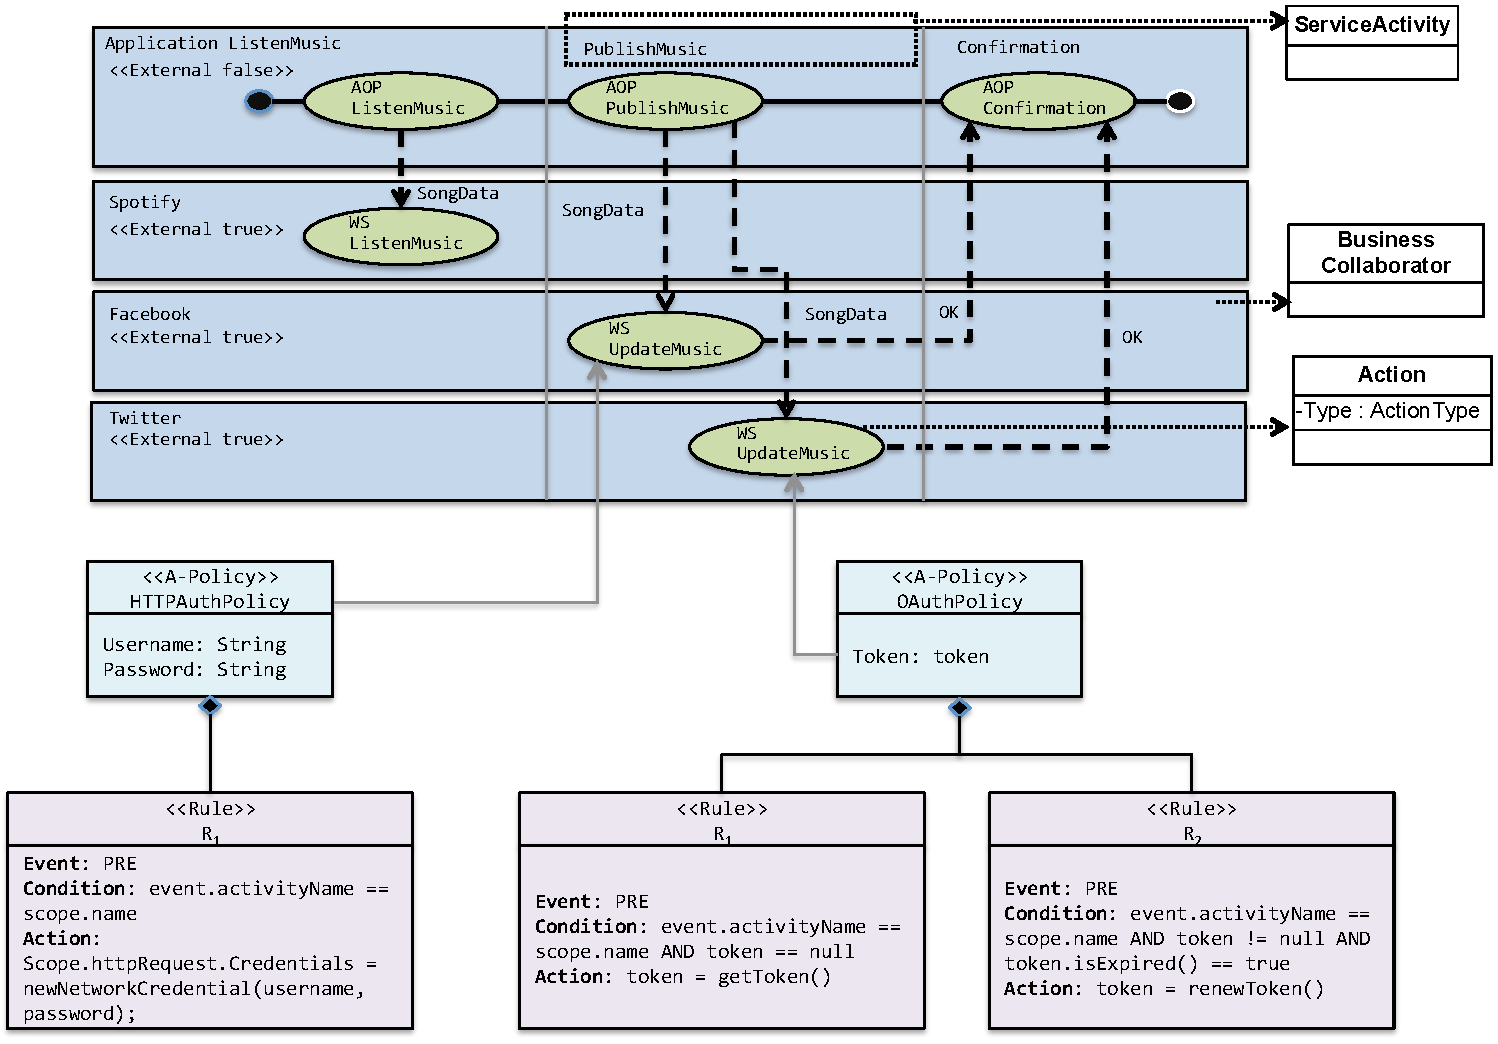
\includegraphics[width=0.95\textwidth]{figs/e-composition-model}
%{\color{red}\LARGE PLACIDO: Please change the names of the boxes in accordance to the explanation --Martin}
\caption{$\pi$-SCM for the ``To publish music'' business service.}
\label{fig:servicecompositionmodel}
\end{figure}

\begin{example}[To Publish Music \textit{(cont)}]\label{ex:toPublicMusic4}
To illustrate the use of the $\pi$-Service Composition meta-model, we define a model for the ``To Publish Music'' scenario (Figure \ref{fig:servicecompositionmodel}). 
 We model a business process that consists of three service activities: {\em Listen Music}, {\em Publish Music} and {\em Confirmation}. 
The {\em Publish Music} activity calls the {\em Facebook} and {\em Twitter} services.
Both {\em Facebook} and {\em Twitter} require authentication. 
Two authentication policies are required, one for {\em Twitter} and another for {\em Facebook}.
%{\color{red} To be completed!.}
In this model, there are three external business collaborators ({\em Spotify, Twitter} and {\em Facebook}).
% \footnote{We use {\em italics} to refer to concrete values of the classes of a model that are derived from the classes of a meta-model.}). 
The model also shows the business process of the application that consists of three service activities: {\em Listen Music}, {\em Publish Music} and {\em Confirmation}. 
Note that  the activity {\em Publish Music} calls the actions of two service collaborators namely {\em Facebook} and {\em Twitter}.
Both {\em Facebook} and {\em Twitter} services require authentication protocols in order to execute methods that will read and update the user space. 
%A call to such services must be part of the authentication protocol required by these services.
In the example, we  associate two authentication policies, one for the open authentication protocol, represented by the class {\sf\small OAuthPolicy} at {\em Twitter}, that will be associated to the activity  {\sf\small UpdateTwitter} (see Figure \ref{fig:servicecompositionmodel}). 
In the same way, the {\em Facebook} class {\sf\small HTTPAuthPolicy}, for the http authentication protocol will be associated to the activity {\sf\small UpdateFacebook}.
{\sf\small OAuthPolicy} will implement the open authentication protocol.
The {\em A-policy} {\sf\small OAuthPolicy} has a variable {\sf\small Token} that will be used to store the authentication token provided by the service.
This variable is imported through the library {\sf\small OAuthPolicy.Token}. 
The A-policy {\sf\small OAuthPolicy} defines two rules, both can be triggered by events of type {\sf\small ActivityPrepared}: (R$_1$): If no token has been associated to the variable {\sf\small token}, then a token is obtained ; and (R$_2$): if the token has expired, then it is renewed. 
Notice that the code in the actions profits from the imported {\sf\small OAuthPolicy.Token} for transparently obtaining or renewing a token from a third party.
{\sf\small HTTPAuthPolicy} implements the HTTP-Auth protocol. 
The A-policy imports an http protocol library and it has two variables {\sf\small username} and {\sf\small password}.  
The event of type {\sf\small ActivityPrepared} is the triggering event of the rule {\sf\small R$_1$}. 
On the notification of an event of that type, a credential is obtained using the username and password. 
\hfill\openbox
\end{example}

%We propose the use of rules and policies to model and associate non-functional properties to service compositions.
%These artifacts will be used to generate the actual programs that will implement the application:
Once the $\pi$-Service Composition Model has been defined, then it can be transformed into a lower level model (in our case, $\pi$-PEWS) that gives support to code generation. 
The $\pi$-PEWS  meta-model is described in the next section. 


%. . - -. . - -. . - -. . - -. . - -. . - -. . - -. . - -. . - -. . - -. . - -. . - -. . - -. . - -. . - -. . - -. . - -. . - -. . - -. . - -. . - -. . - -. . - -. . - -. . - -. . - -
\subsection{Platform Specific Models}
%. . - -. . - -. . - -. . - -. . - -. . - -. . - -. . - -. . - -. . - -. . - -. . - -. . - -. . - -. . - -. . - -. . - -. . - -. . - -. . - -. . - -. . - -. . - -. . - -. . - -. . - -

This level focusses on the functionality, in the context of a particular implementation platform.
Models at this level combine the platform-independent view with the specific aspects of the platform to implement the system. At the PSM level we have lower-level models that can be automatically translated into actual computer programs. 
We have defined one meta-model at this level.

The \textit{$\pi$-PEWS} meta-model provides concepts for modelling service compositions. 
Instances of this meta-model are textual descriptions of service compositions that can be translated into any service composition language, such as BPEL~\cite{bpel03} or PEWS~\cite{BaCAM05,Placido2010LTPD}.

PEWS~\cite{BHM06,Placido2010LTPD} is a notation to express service compositions.
The language is based on the notion of Path Expressions~\cite{And79} and can easily be translated into any actual composition language, such as BPEL~\cite{bpel03}. 
Figure~\ref{fig:metamodel} presents the $\pi$-{\sc Pews} meta-model, where we identify classes to describe:
\begin{itemizedTrivlist}
\item Service compositions: {\sc Namespace} representing the interface exported by a service, {\sc Operation} that represents a call to a service method, {\sc CompositeOperation}, {\sc Operator} and {\sc Path} for representing service compositions.
A {\sc Path} can be an {\sc Operation} or a {\sc Compound Operation}. 
A {\sc Compound Operation} is defined using an {\sc Operator}.
The language defines operators to denote guarded operations ($[C]S$); sequential ($\ . \ $), parallel ($\ \| \ $) and alternative ($\ + \ $) compositions; as well as sequential ($*$) and parallel ($\{\dots\}$) repetition.

\item {\em A-Policies} that can be associated to a service compositions:  {\sc A-Policy}, {\sc Rule}, {\sc Event}, {\sc Condition}, {\sc Action}, {\sc State}, and {\sc Scope}.
A brief description of these classes is given next.
\end{itemizedTrivlist}
%
\begin{figure}[t]
\centering
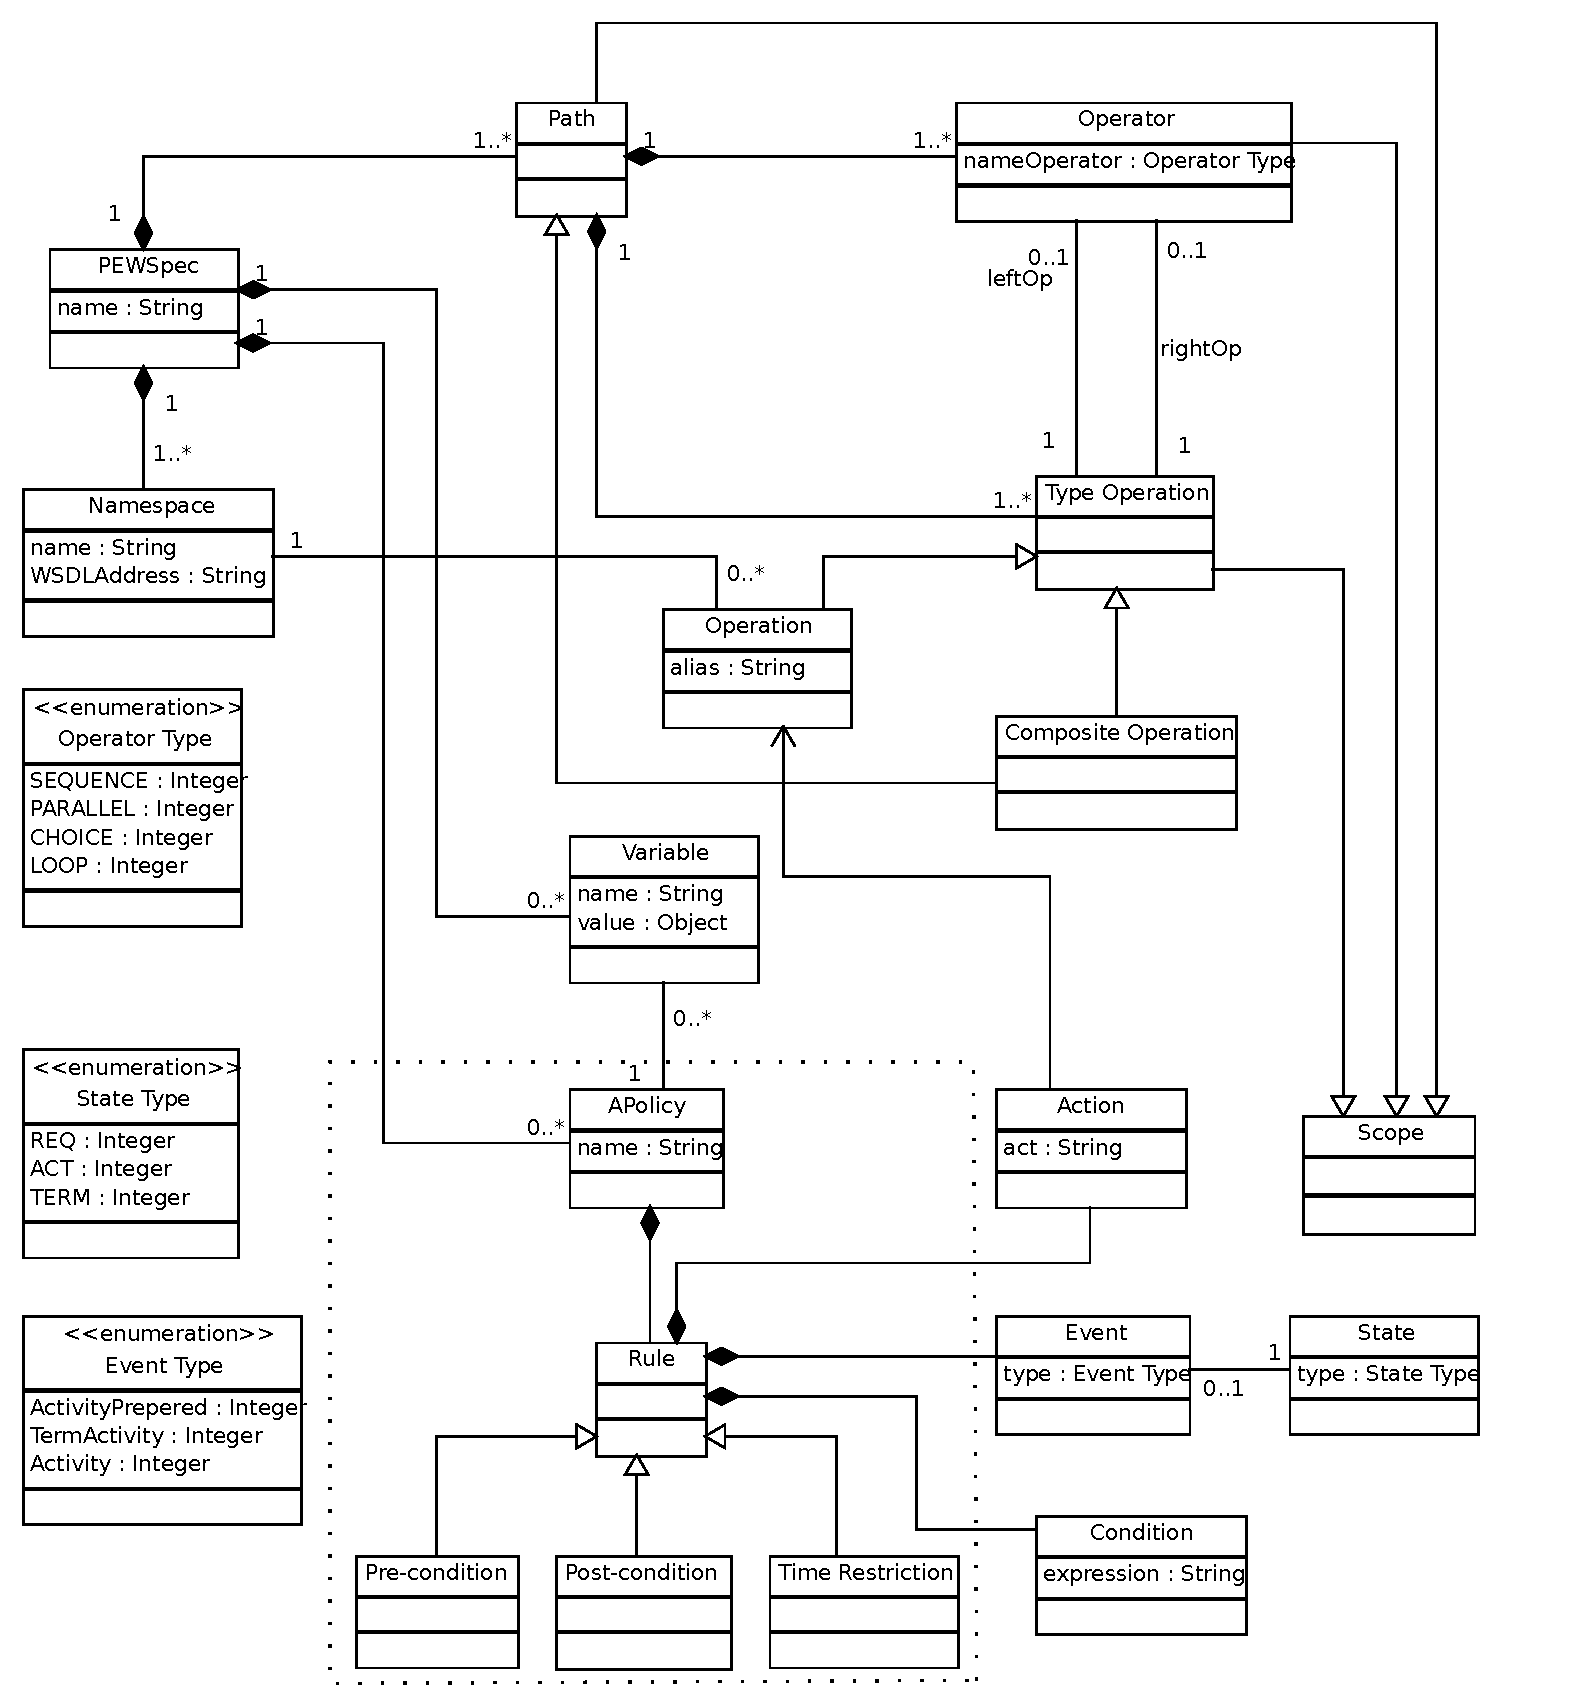
\includegraphics[width=1.0\textwidth]{figs/PEWSMetamodel}
\caption{$\pi$-{\sc Pews} Metamodel}
\label{fig:metamodel}
\end{figure}

Figure~\ref{fig:metamodel} shows that each {\sc A-Policy} is associated to a {\sc Scope} that can be either an {\sc Operation} (e.g., an authentication protocol associated to a method exported by a service),  an {\sc Operator} (e.g., a temporal constraint associated to a sequence of operators) or a {\sc Path}.  
Each {\sc A-Policy} groups a set of ECA rules with a classic semantics, i.e, {\em when an event of type E occurs, if condition C is verified then execute the action A}.  
In this way, an {\em A-policy} represents a set of reactions to be possibly executed when one or several events are notified.

Given a $\pi$-SCM model of a specific service based application (expressed according to the $\pi$-SCM meta-model), it is possible to generate its corresponding $\pi$-{\sc Pews} model. 
The following section describes the transformation rules between the $\pi$-SCM and $\pi$-{\sc Pews} meta-models.



%..--..--..--..--..--..--..--..--..--..--..--..--..--..--..--..--..--..--..--..--..--..--..--..--..--..--..--..--..--..--..--..
%\subsubsection{$\pi$-{\sc Pews}  meta-model}\label{sec:pewsmetamodel}
%..--..--..--..--..--..--..--..--..--..--..--..--..--..--..--..--..--..--..--..--..--..--..--..--..--..--..--..--..--..--..--..

%..--..--..--..--..--..--..--..--..--..--..--..--..--..--..--..--..--..--..--..--..--..--..--..--..--..--..--..--..--..--..--..--..--..--..--..--..--..--
\section{Transformation rules}\label{sec:mmrules}
%..--..--..--..--..--..--..--..--..--..--..--..--..--..--..--..--..--..--..--..--..--..--..--..--..--..--..--..--..--..--..--..--..--..--..--..--..--..--

 $\pi$-SOD-M  proposes  horizontal transformation rules between $\pi$-use case to $\pi$-service process models,  and vertical transformation rules between $\pi$-service process to $\pi$-service composition  models; and $\pi$-service composition model to $\pi$-PEWS code. The following lines describe the particular purpose of these transformation rules that are intended to (semi)-automatize the construction of a service oriented application (see the $\pi$-SODM environment description in the next section).
 
% _ . _ . _ . _ . _ . _ . _ . _ . _ . _ . _ . _ . _ . _ . _ . _ . _ . _ .
\subsection{From $\pi$-UseCase to the $\pi$-ServiceProcess}
% _ . _ . _ . _ . _ . _ . _ . _ . _ . _ . _ . _ . _ . _ . _ . _ . _ . _ .

Given  (composite) $\pi$-use case model defining the functions of  the developed application and their associated constraints (representing business rules), the objective is to express them as a $\pi$-service process model describing the application logic and its associated non-functional properties.  The principle is to express a set of $\pi$-use cases (i.e., use cases with constraints) related by relationships of type {\sc Extend}   in terms of  a business process consisting of actions related by a control flow and associated contracts specifying NFP. The PIM to PIM transformation rules specify how  to transform a $\pi$-use case model into  a $\pi$-service process model.
%(Table \ref{fig:transformationsUseCase-ServiceProcess}). 

%\begin{figure}
%\centering{
%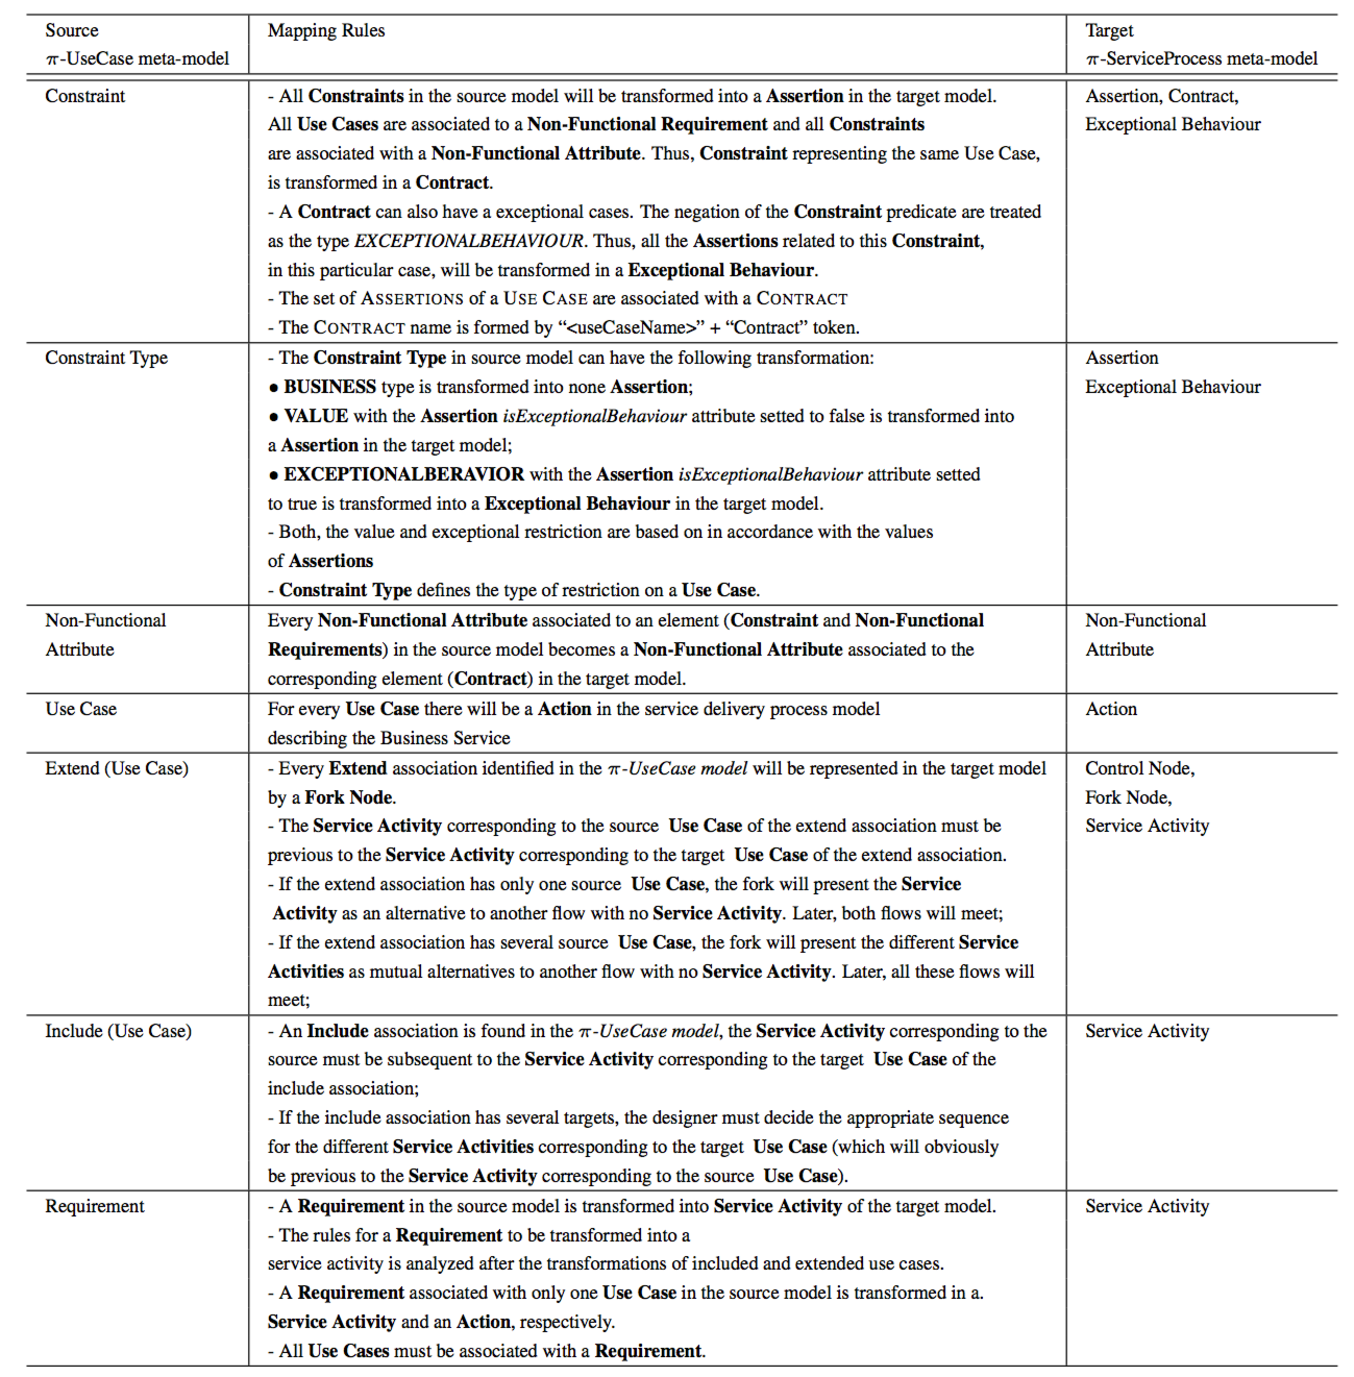
\includegraphics[width=0.96\textwidth]{figs/Table5}}
%\caption{ $\pi$-UseCase to $\pi$-ServiceProcess transformation}
%\label{fig:transformationsUseCase-ServiceProcess}
%\end{figure}

As defined in the $\pi$-ServiceProcess  meta-model an {\sc Activity service}  consists of a composition of  entities of type {\sc Action}. 
Thus, every {\sf $\pi$-use case} is transformed into an {\sf Action} of the target $\pi$-service process model.  Every {\sf Extend} relationship identified in a $\pi$-use case model is transformed into a  {\sf Fork node}.
If the {\sf Extend} relationship concerns: 
\begin{itemize}
\item one {\sf use case} it is transformed into an {\sf Action} participating in the fork node in an alternative flow. 
\item several  {\sf use cases} are transformed as  different {\sf Actions} that belong to mutual alternative flows in the fork node.   
%{\sc Contracts}  are associated to  {\sc Actions}.
\end{itemize}

\begin{figure}
\centering{
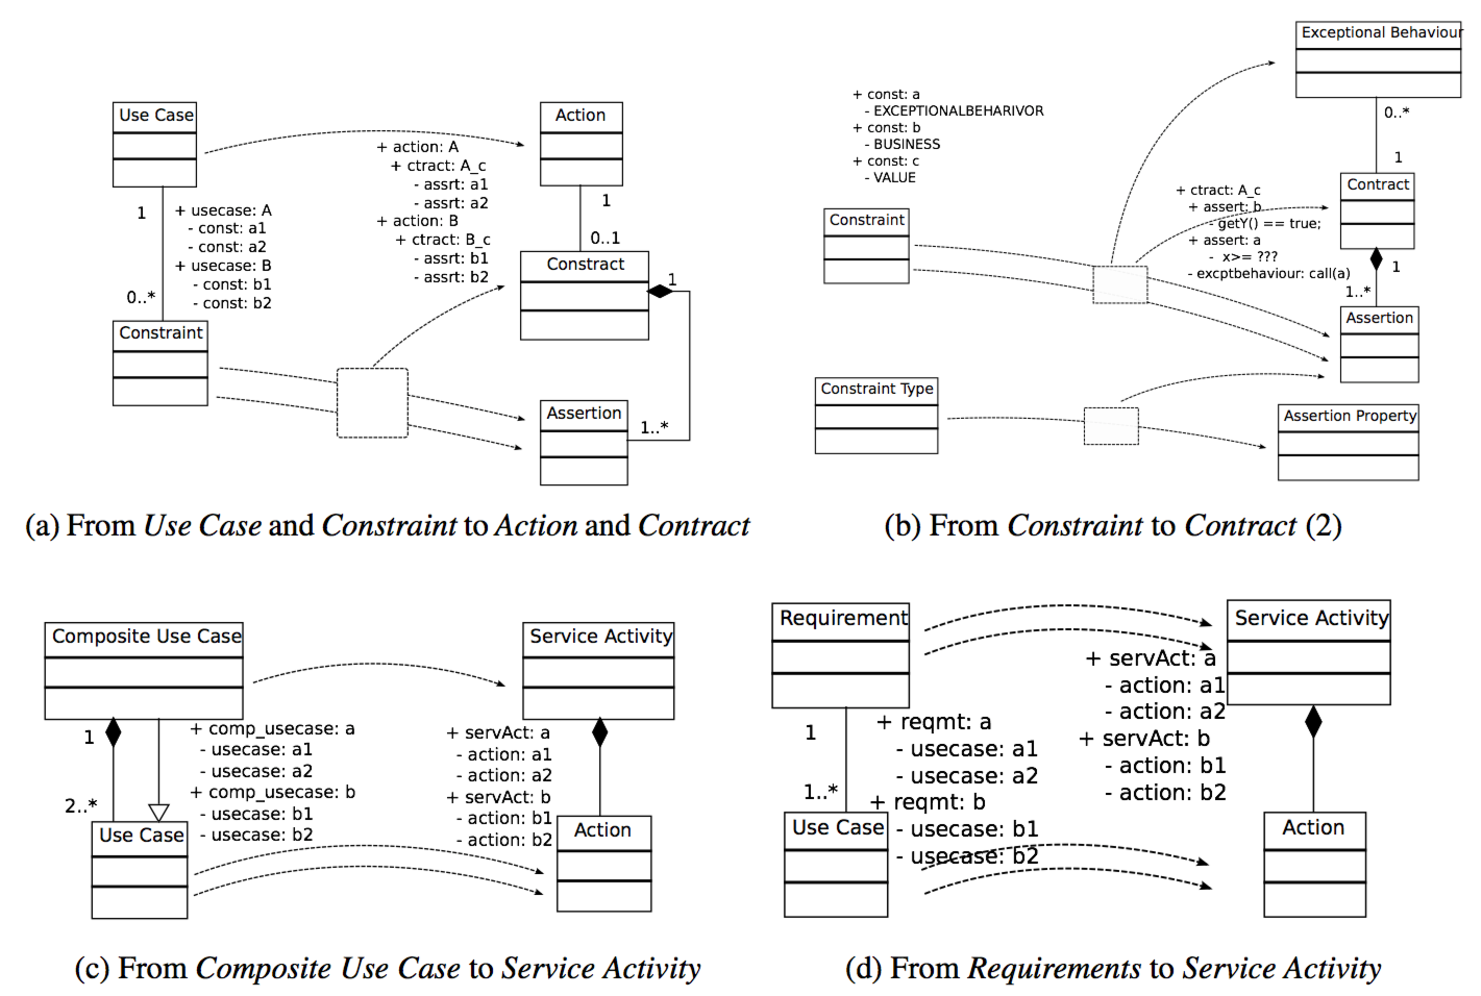
\includegraphics[width=0.96\textwidth]{figs/35}}
\caption{ $\pi$-UseCase to $\pi$-ServiceProcess transformation rules}
\label{fig:transformationsUseCase-ServiceProcessRules}
\end{figure}

   A {\sf Constraint} of a (composite) {\sf Use Case}  is transformed into an  {\sf Assertion}.  The set of constraints  in a $\pi$-use case model  (transformed into assertions) are grouped in a {\sf Contract} in a $\pi$-service process model (figure  \ref{fig:transformationsUseCase-ServiceProcessRules}-a).
A constraint of a given type ({\sf Constraint type}) can have different transformations as stated in the following rules (figure   \ref{fig:transformationsUseCase-ServiceProcessRules}-b). Given a  a {\sf Constraint} of type:

\begin{itemize}
\item   {\sc Business} is transformed into an {\sf Assertion} with no value attributes. %information like maxValue and minValue;
\item     {\sc Value}  with the  attribute {\sf  isExceptionalBehaviour}  set to false, is transformed into an {\sf Assertion}.
\item  {\sc Value }  with the attribute {\sf  isExceptionalBehaviour }  set to true, is transformed into  {\sf Exceptional behaviour}.
\end{itemize}
%Given the $\pi$-UseCase meta-model, to all {\sc Constraint} entity related with a {\sc Use Case}, there is a {\sc Contract} that compounds a set of {\sc Assertions} entity  and the {\sc Use Case} is refined in a service {\sc Action}.


 For transforming constraints of type {\sf Value Constraint }
  the designer must specify value thresholds associated to attributes as specified by  { constraint}s  and {use case}s. By default, value constraints are transformed into pre-conditions and business constraints are transformed into post-conditions. 
  

% From {\sc Constraint} and {\sc Constraint Type} entities are generated detailed {\sc Contract} information, that are refined into {\sc Exceptional behaviours} and {\sc Assertions} entities . {\sc Constraint} is related with a {\sc Constraint type}, and there are different cases for the transformation of this concept. A Business type is transformed into an {\sc Assertion} . These {\sc  Assertion} information attributes are considered if the {\sc Constraint Type} is a Value type. This is semi-automatic, because there is not
%enough information in a $\pi$-UseCase model to run a complete automatic transformation. 

A {\sf Requirement} and a {\sf Composite use case} in a  $\pi$-UseCase model are transformed respectively into a {\sf Service activity} and an {\sf Action} (see figures  \ref{fig:transformationsUseCase-ServiceProcessRules}-c  and d). 


\begin{figure}
\centering{
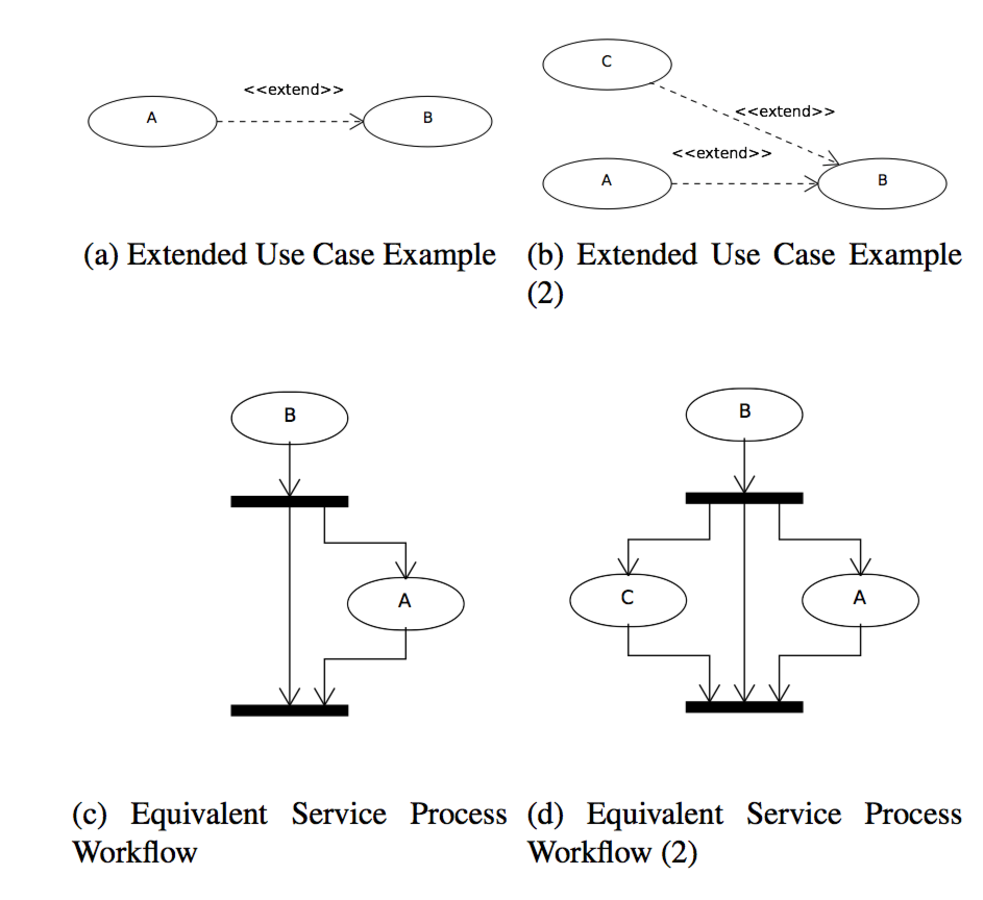
\includegraphics[width=0.80\textwidth]{figs/37}}
\caption{ Extended Transformation Examples}
\label{fig:transformaton-examples}
\end{figure}

%The transformations for {\sc Extend} and {\sc Include} dependencies  are not as simple as the previous transformations (figures \ref{fig:transformaton-examples}-a). 

The relationships of type  {\sc Extend} and {\sc Include}  determine the way the business process is expressed as a workflow.  The workflow generated for a relationship  �extends�  between  two use cases (figure  \ref{fig:transformationsUseCase-ServiceProcessRules}-a) is described in figure \ref{fig:transformaton-examples}-c).  The generated workflow consists of  a {\sf Fork node}, a {\sf Join node},  four entities of type {\sc Control flow}, and also two entities of type {\sc Action} , one for each {\sf Use case}.

When there is more than one �extends� relationship among several use cases (figures \label{fig:transformationsUseCase-ServiceProcessRuless}-b), the transformation leads to  two more {\sc Control flow} entities for each  {\sc use case}, and an {\sf Action} for each  extended {\sf use case}.



\begin{figure}
\centering{
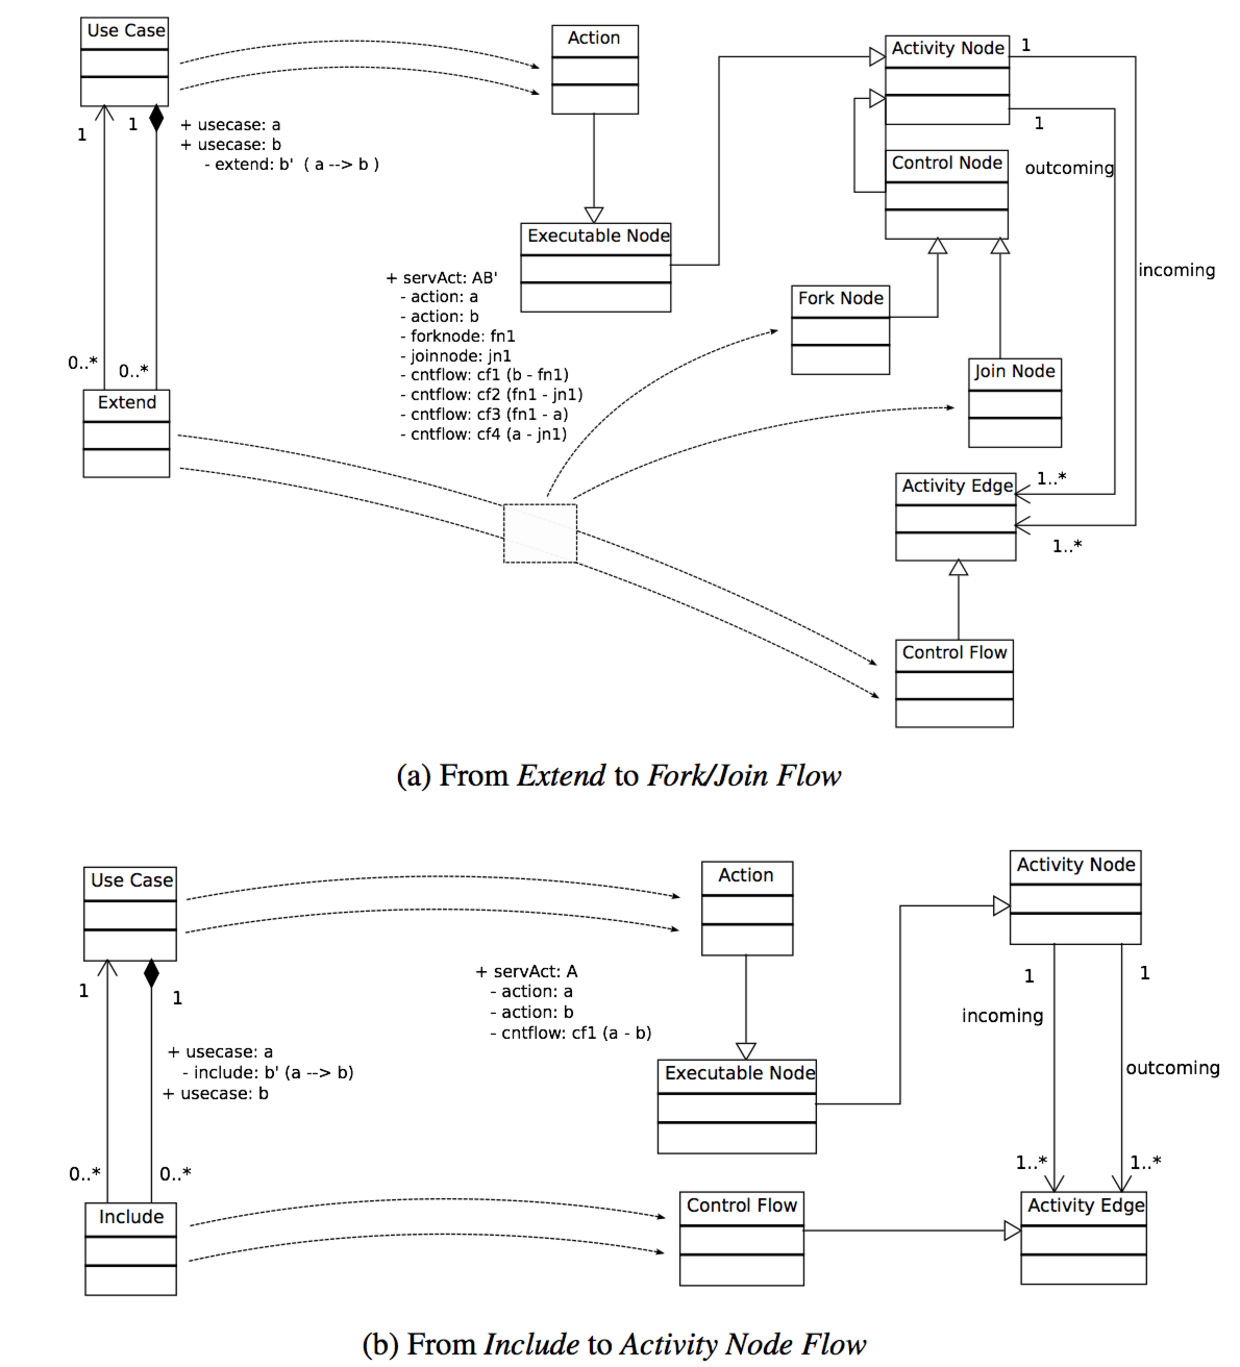
\includegraphics[width=0.96\textwidth]{figs/36}}
\caption{ $\pi$-UseCase to $\pi$-ServiceProcess Model Transformation Rules (2)}
\label{fig:transformationsUseCase-ServiceProcessRules}
\end{figure}

 {\sf Include} use case entities, are transformed into an {\sf Action} sequence, as shown in figure \ref{fig:transformationsUseCase-ServiceProcessRules}-b. A {\sc Use case} element is transformed into an {\sf Action}. A set of n {\sc Use case} is transformed into an  n-1 {\sf Object flow} elements. Each {\sf Control flow} is transformed into two {\sf Actions} associated by a relationship.

\begin{example}[To Publish Music \textit{(cont)}]\label{ex:toPublicMusicT1}
Considering the scenario example  the transformation of the "listen music" Use Case is transformed into a Service Action. This Action  represents a Spotify service function that can be invoked to play the music. For the "publish music" use case,  constraints are transformed in a set of assertions that are grouped in a Contract ({\sf "publishMusicContract"}) associated to the Action {\sf "publishMusic"}. 
The "download music" use case  includes the payment process to buy the music. Thus, these use cases  are transformed into {\sf Actions}, and a {\sf Service activity} that aggregates these {\sf Actions}.   It is transformed in a sequence flow in the $\pi$-service process model (as shown in figure \ref{fig:transformation-example-include}). 
The same rule is applied for the "publish music" use case, which has two extended use cases, "public twitter" and "public Facebook" (figures \ref{fig:transformaton-examples}-b and d).
 \end{example}

%\begin{figure}
%\centering{
%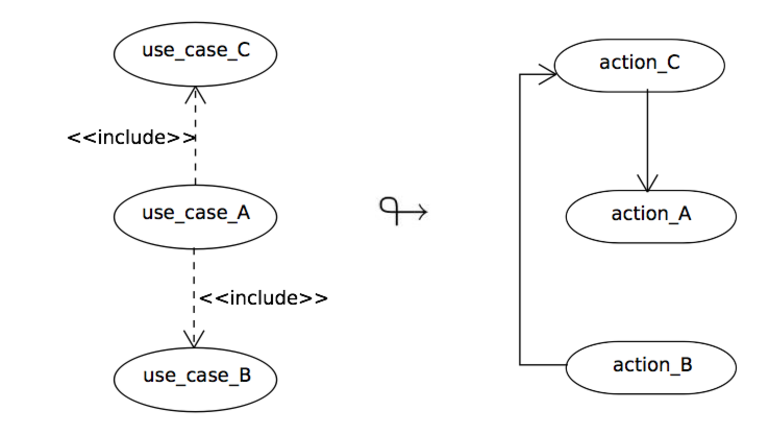
\includegraphics[width=0.76\textwidth]{figs/38}}
%\caption{ Include Transformation Example}
%\label{fig:transformation-example-include}
%\end{figure}

% _ . _ . _ . _ . _ . _ . _ . _ . _ . _ . _ . _ . _ . _ . _ . _ . _ . _ .
\subsection{From $\pi$-ServiceProcess to $\pi$-ServiceComposition}
% _ . _ . _ . _ . _ . _ . _ . _ . _ . _ . _ . _ . _ . _ . _ . _ . _ . _ .
%The {\em A-policies} defined for the elements of the $\pi$-SCM are transformed into {\sc A-Policy} classes, named according to the names expressed in the source model. The transformation of the rules expressed in the $\pi$-SCM is guided by the event types associated to these rules.   The variables associated to an {\em A-policy} expressed in the $\pi$-SCM as {\sc\em $<$Variable:name, Variable:type$>$} are transformed into elements of type {\sc Variable} with attributes {\sc name} and {\sc type} directly specified from the elements {\sc\em  Variable:name} and {\sc\em Variable:type} of the $\pi$-SCM model.

%As shown in Figure \ref{fig:transformations}, for an event of type {\sc\em Pre} the corresponding transformed rule is of type {\sc Precondition}; for an event of type {\sc\em Post} the corresponding transformed rule is of type {\sc Postcondition}; finally, for an event of type {\sc\em TimeRestriction} the corresponding transformed rule is of type {\sc Time}. 
%The condition expression of a rule in the $\pi$-SCM ({\sc\em Rule:condition}) is transformed into a class {\sc\em Condition:expression} where the attributes of the expression are transformed into elements of type {\sc Attribute}.

%The attribute event of a rule  ({\sc\em Rule:event}) in the $\pi$-SCM is transformed into an {\sc Event Type} according to the rule type. 

%As shown in Figure \ref{fig:transformations}, the event type for a rule of type (i) {\sc Precondition} is {\sc ActivityPrepared}; (ii) {\sc Postcondition} is {\sc TermActivity}; (iii) {\sc TimeRestriction} is {\sc Temporal}. The {\sc\em Rule:Action} of a rule in the $\pi$-SCM is transformed into an {\sc Action:type}.

%
%Figure \ref{fig:p-scim} shows the  $\pi$-{\sc Pews} model for our example.
%In the scenario "To Publish Music" the {\sf Policies} {\em OAuthPolicy} and {\em HTTPAuthPolicy} of the $\pi$-SCM model are transformed into {\em A-policies} of type {\sf Precondition} of the $\pi$-{\sc Pews} model of the scenario. Thus in both cases the events are of type {\sf ActivityPrepared}. These policies, as stated in the $\pi$-SCM model, are associated to {\sf Activities}. In the corresponding transformation they are associated to {\sf Operation}s {\em PublishFacebook} and {\em PublishTwitter}.
%\begin{figure}[htpb]
%\centering{
%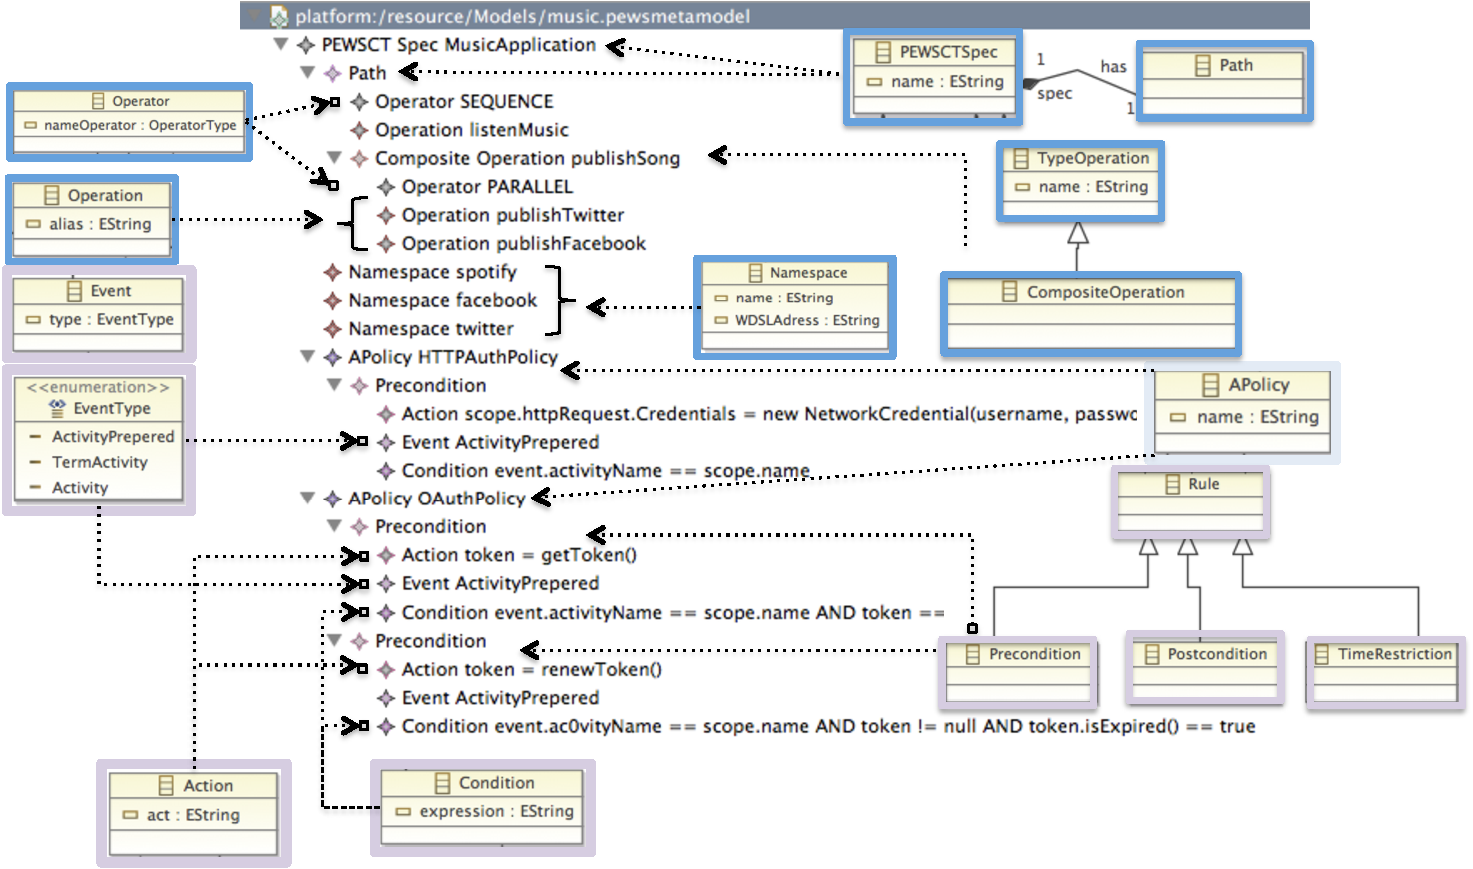
\includegraphics[width=0.78\textwidth]{figs/modeloPEWS}}
%\caption{$\pi$-{\sc Pews} generated model fo the "To Publish Music" application}
%\label{fig:p-scim}
%\end{figure}

%Figure \ref{fig:pewsexpression} shows the correspondence between the model and the statements that implement it, with a schematic representation of the business process.
%\begin{figure}
%\centering{
%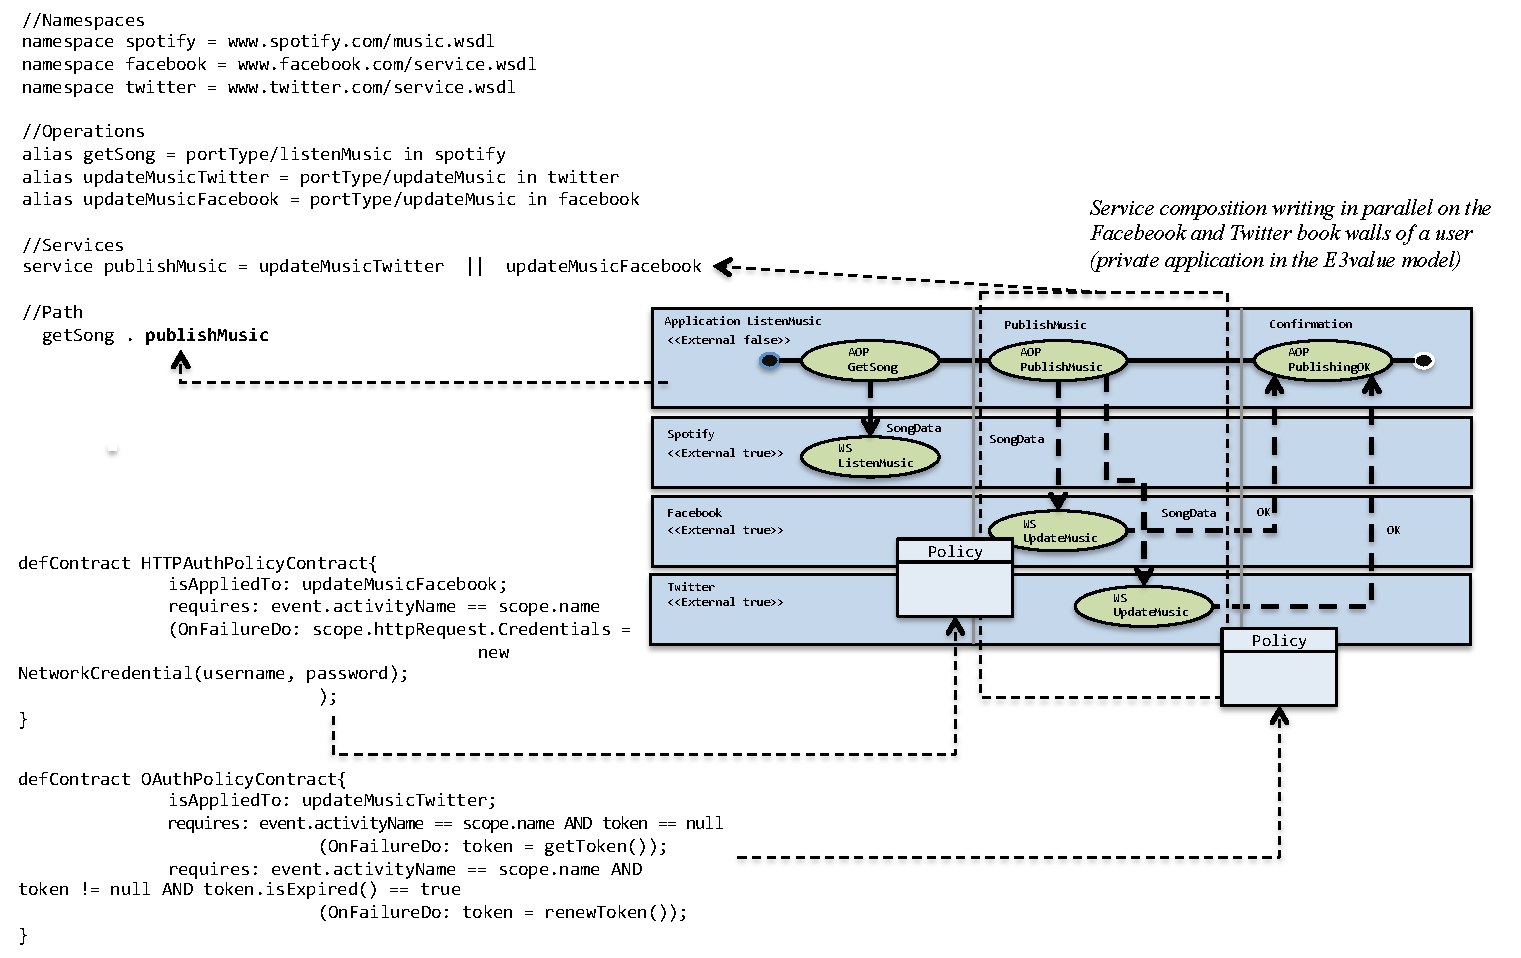
\includegraphics[width=0.85\textwidth]{figs/pews-expression}}
%\caption{Pews program implementing the "To Publish Music" application}
%\label{fig:pewsexpression}
%\end{figure}
%Table \ref{fig:ServiceProcess-ServiceComposition}  shows the transformation rules for transforming a .
As illustrated in Figure \ref{fig:ServiceProcess-ServiceComposition-Rules} the  principle of the transformation  of a  $\pi$-Service process model into a   $\pi$-ServiceComposition model is to group respectively  {\sf Contracts}  and {\sf Actions} into {\sf Policies} and {\sf Service activities}.   

Each {\sf Assertion} of a {\sf Contract} in a $\pi$-service composition model is transformed into a {\sf Rule} in a $\pi$-service composition model. The set of {\sf Rules}  concerning the same NFP (e.g., safety, performance, and reliability) is grouped into a {\sf Policy} (see Figure \ref{fig:ServiceProcess-ServiceComposition-Rules}-a). Each {\sf Assertion} of a {\sf Contract} is transformed into a {\sf Rule:Condition} attribute. If the {\sf Assertion} has a value type, the name and the attributes are transformed into a {\sf Variable} in the target model.  The {\sf Assertion: Aproperty} attribute can have different transformations, according to  the following rules:
\begin{itemize}
\item a {\sf Post-Condition} is transformed into a {\sf  Post}. 
\item a {\sf Precondition} is transformed into {\sf Pre}.
\item a {\sf Timerestriction} is transformed into {\sf Time}.
\end{itemize}


\begin{figure}
\centering{
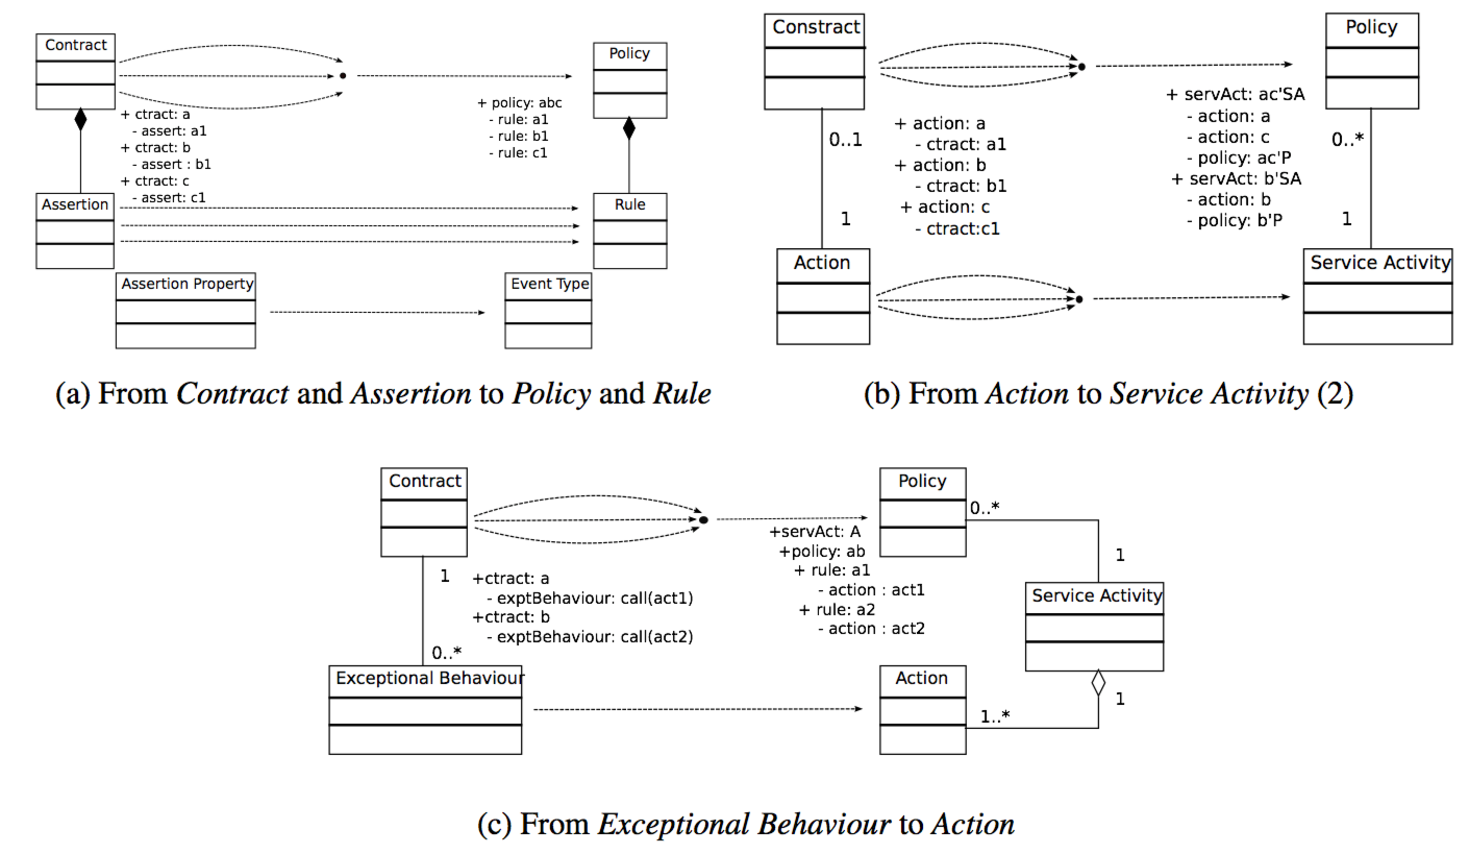
\includegraphics[width=0.96\textwidth]{figs/ExceptionalRules}}
\caption{$\pi$-ServiceProcess to $\pi$-ServiceComposition Model Transformation Rules}
\label{fig:ServiceProcess-ServiceComposition-Rules}
\end{figure}

A {\sf Package}  in the $\pi$-use case model is transformed   into a {\sf Business Collaborator}. 
{\sf Actions}  of a $\pi$-service process model are transformed into an {\sf Action} in a $\pi$-service composition model, and every {\sf Service activity} of a $\pi$-service process model is transformed into a {\sf Service activity} in a $\pi$-service composition model (see Figure \ref{fig:ServiceProcess-ServiceComposition-Rules}-b). An {\sf Exceptional behaviour} entity is transformed into an {\sf Action} in a $\pi$-service composition model (see Figure \ref{fig:ServiceProcess-ServiceComposition-Rules}-c ), and every {\sf Non-functional attribute} associated to an element ({\sf Contract} and {\sf Non-functional requirement}) in a $\pi$-service process model becomes a {\sf Non-functional attribute} associated to the corresponding element {\sf Policy} in a $\pi$-service composition model.
 Finally, {\sf Actions} are grouped by  a  {\sf Business collaborator}.  

%\begin{figure}
%\centering{
%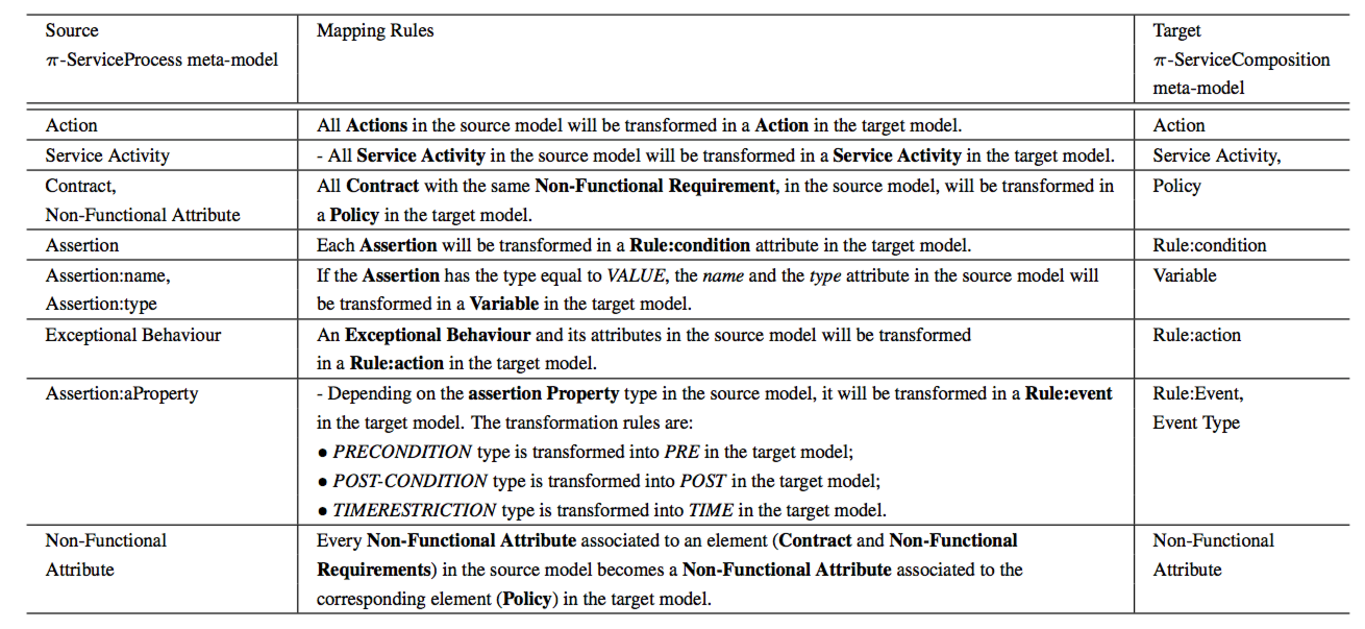
\includegraphics[width=1\textwidth]{figs/ServiceProcess-ServiceComposition}}
%\caption{ Transformation Rules: From $\pi$-ServiceProcess to $\pi$-ServiceComposition}
%\label{fig:ServiceProcess-ServiceComposition}
%\end{figure}






%As the $\pi$-ServiceComposition model refines the $\pi$-ServiceProcess concepts at PIM level, a service previously defined as actions (source model) is refined as composition of those actions (target model) that are necessary to represent a business service, identifying who are the partners involved in the realization ({\sc Business collaborators}). 
%In addition, $\pi$-SOD-M defines a platform specific model based on web services composition. This model is explicitly indicates those actions which are (or will be, if not yet implemented) supported by web services.

\begin{example}[To Publish Music \textit{(cont)}]\label{ex:toPublicMusicT5}
Considering the scenario example, 
%the {\sf Action}s update music {\sc Contract} is transformed is a {\sc Policy} with its {\sc Rules}. All contract {\sc Assertions} are transformed in RULE and its attributes, e.g. the login and password verification. 
the "securityLoginPolicy" consists of a set of {\sf Rules} that were transformed from the {\sf Assertions} in $\pi$-service process model. 
%The {\sc Non- functional requirement} information will be used to the {\sc Policy} generation comes from the initial use case model. Also 
The {\sf Business Collaborator} Facebook and Spotify information come from entity of type {\sc Package}  in the $\pi$-use case model. 
%All {\sc Contracts} of the same {\sc Non- functional requirement} are composed in a {\sc Policy}.
\end{example}

% _ . _ . _ . _ . _ . _ . _ . _ . _ . _ . _ . _ . _ . _ . _ . _ . _ . _ .
\subsection{From $\pi$-ServiceComposition to $\pi$-PEWS}
% _ . _ . _ . _ . _ . _ . _ . _ . _ . _ . _ . _ . _ . _ . _ . _ . _ . _ .

%Table \ref{fig:ServiceComposition-Pews-Rules} 
This section describes the PIM to PSM transformations between a $\pi$-Service composition and a $\pi$-PEWS program. We propose two groups of rules: those that transform services composition entities of a $\pi$-Service composition model into $\pi$-PEWS model ; and those that transform rules grouped by policies into A-policy types.

A named action of the $\pi$-service composition model represented by  {\sf Action} and {\sf Action:name} is transformed to an  {\sf Operation} with a corresponding attribute name {\sf Operation:name}. A  named service activity represented by the elements {\sf ServiceActivity}  and  {\sf ServiceActivity:name} of the $\pi$-service composition model, are  transformed into a named operation of the $\pi$-{Pews} represented by the entities  {\sf CompositeOperation} and {\sf CompositeOperation:name}. When more than one action is called, according to the following  composition patterns expressed using the operators {\sc\em merge, decision, fork and join} in the $\pi$-service composition model the corresponding transformations, according to the PEWS operators presented above:
\begin{itemize}
\item   $op_1 . op_2$ if no {\sc\em ControlNode} is specified
\item ($op_1 \parallel op_2) . op_3$ if control nodes of type {\sc\em fork, join} are combined
 \item ($op_1 + op_2) . op_3$ if control nodes of type {\sc\em decision, merge} are combined
\end{itemize}

%\begin{figure}
%\centering{
%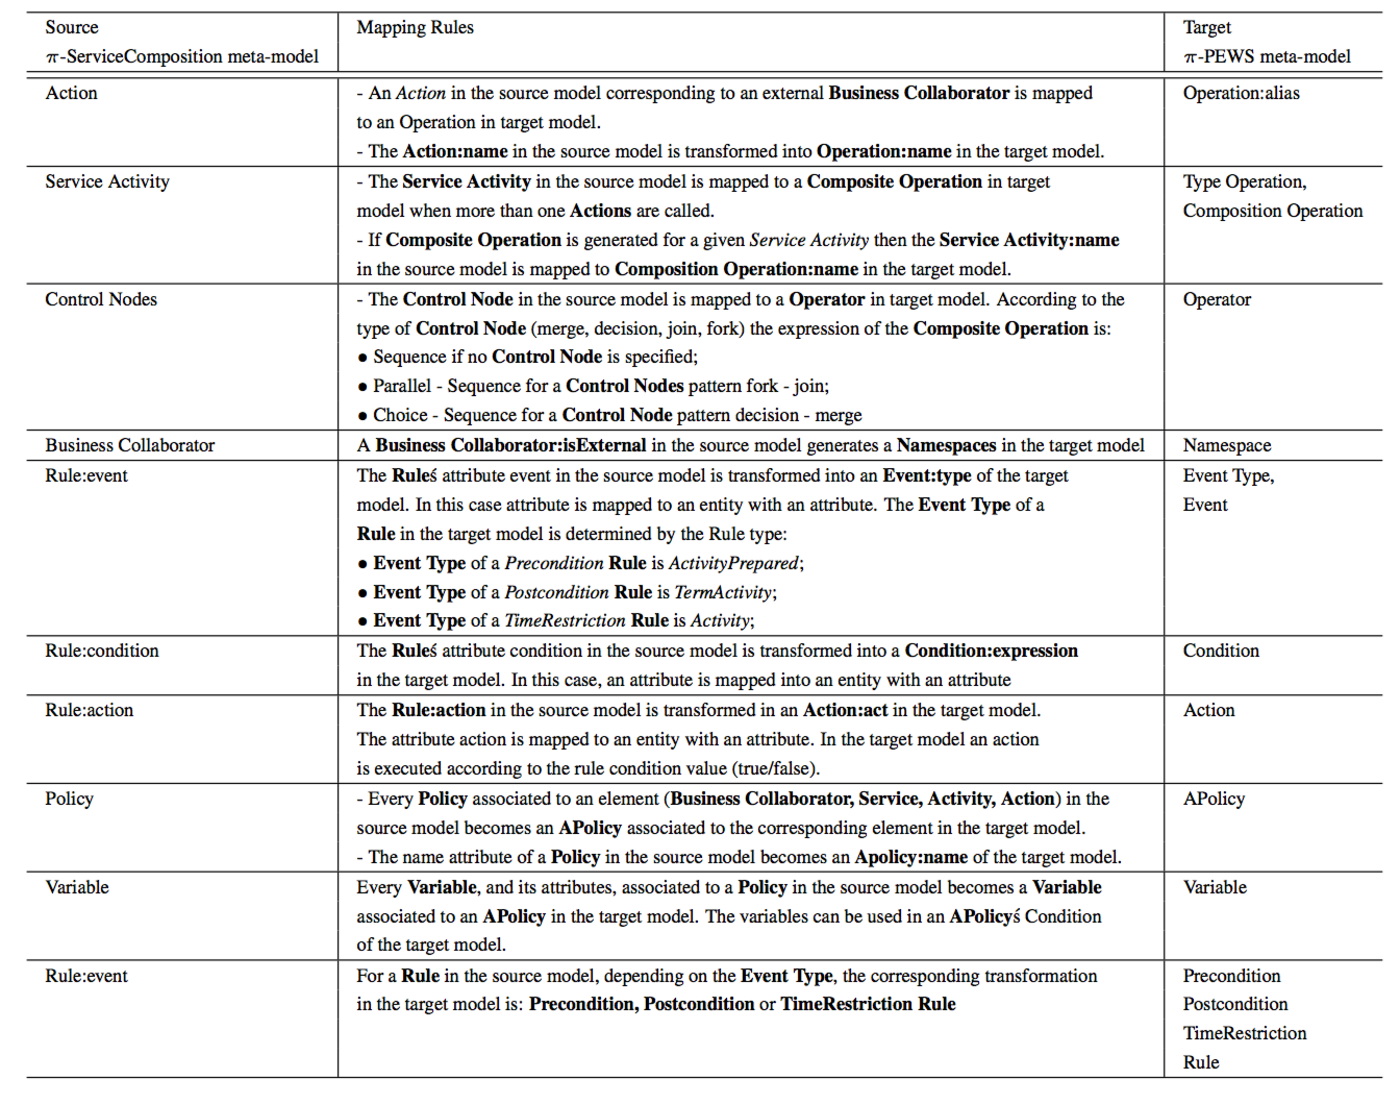
\includegraphics[width=0.96\textwidth]{figs/Table7}}
%\caption{Transformation Rules: From $\pi$-ServiceComposition to $\pi$-PEWS}
%\label{fig:ServiceComposition-Pews-Rules}
%\end{figure}


The A-policies defined for the entities of a $\pi$-service composition model are transformed into {\sf A-policy} entities, named according to the names expressed in the source model. The transformation of the rules expressed in a $\pi$-service composition is guided by the event types associated to these rules. The variables associated to an A-policy expressed in a $\pi$-service composition model as {\sf $<$Variable:name, Variable:type$>$} are transformed into entities  {\sf Variable} with attributes {\sf Name} and {\sf Type} directly specified from the elements {\sf Variable:name} and {\sf Variable:type} of a $\pi$-service composition model.

%As shown in Table \ref{fig:ServiceComposition-Pews-Rules}, 
For an event of type Pre the corresponding transformed rule is a {\sf Precondition}; for an event of type Post the corresponding transformed rule is a {\sf Post- condition}; finally, for an event of type TimeRestriction the corresponding transformed rule is a {\sf Time}. The condition expression of a rule in a $\pi$-service composition ({\sf Rule:condition}) is transformed into a  {\sf Condition:expression} where the attributes of the expression are transformed into  entities {\sf Attribute}.

Figure \ref{fig:Specific-Contract-Representation} shows the $\pi$-PEWS code resulting from the $\pi$- service composition model  of our scenario example.

\begin{figure}
\centering{
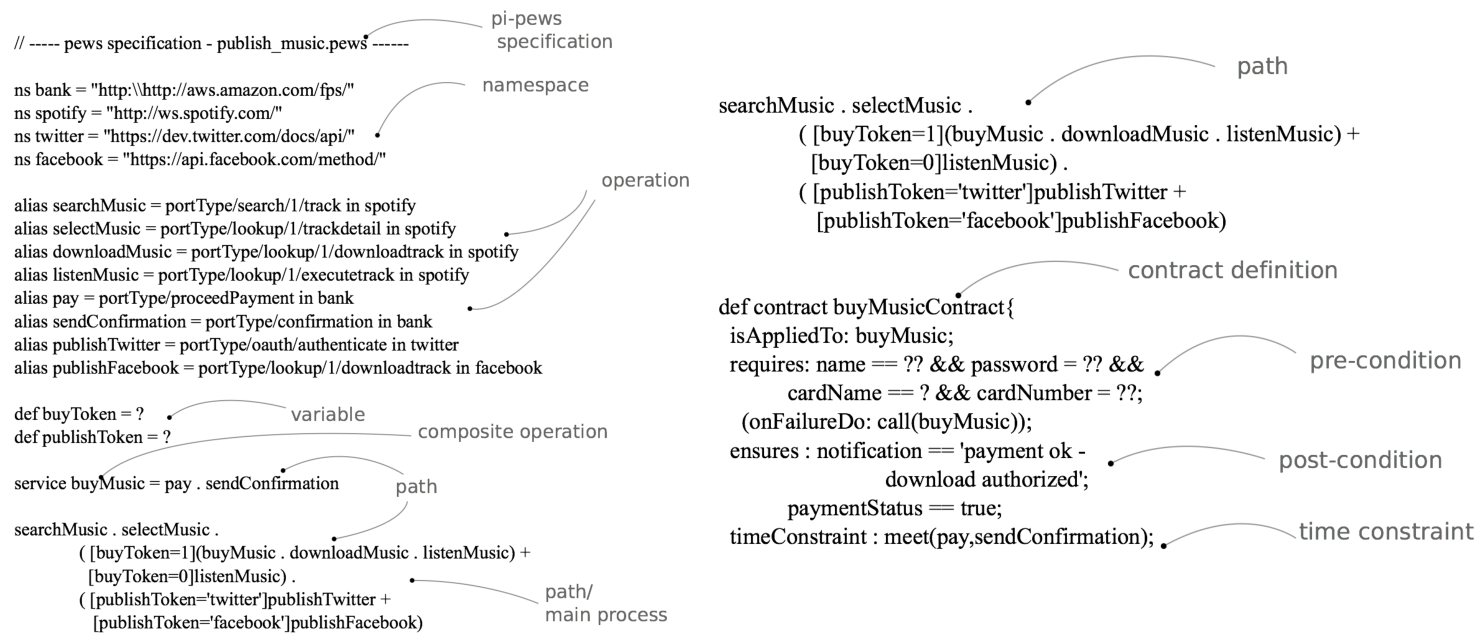
\includegraphics[width=0.96\textwidth]{figs/31-31}}
\caption{$\pi$-PEWS Specific and Contract Representation}
\label{fig:Specific-Contract-Representation}
\end{figure}

